%\documentclass[letterpaper,12pt]{article}
\documentclass[superscriptaddress,preprintnumbers,amsmath,amssymb,aps,11pt]{revtex4}
%\usepackage[]{authblk}
%\usepackage{graphics}
\usepackage[dvipdf]{graphicx}
%\usepackage{subfig}  % For subfloats
\usepackage{color}
\usepackage{multirow}
\usepackage{epsfig}
\usepackage{wrapfig}
\usepackage{rotating}
\usepackage{caption}
\usepackage{subcaption}

\def \rarr {\rightarrow}
\def \grinp {\includegraphics}
\def \tw {\textwidth}
\def\dfrac#1#2{\displaystyle{{#1}\over{#2}}}
\def \dstl {\displaystyle}
\definecolor{GREEN}{rgb}{0.,0.8,0}
\definecolor{RED}{rgb}{1,0,0}
\definecolor{ORANGE}{rgb}{1,0.5,0}
\newcommand{\JLAB}{Thomas Jefferson National Accelerator Facility, Newport News, Virginia 23606}
\newcommand{\ORSAY}{Institut de Physique Nucleaire d'Orsay, IN2P3, BP 1, 91406 Orsay, France}
\newcommand{\UNH}{University of New Hampshire}
\newcommand{\GLASGO}{Glasgow University, Glasgo, Scotland} 
\begin{document}
%\rightline{LOI-PAC43}

\title{Di-muon electroproduction with 11GeV electron beam and the modified CLAS12 detector}

\author{M. Boer} \author{M. Guidal} \author{E. Voutier} 
\affiliation{\ORSAY}
\author{N. Baltzell} 
\author{V. Burkert} 
\author{L. Elouadrhiri} 
\author{F-X. Girod}
\author{P. Nadel-Turonski ...}
\author{S. Stepanyan}
\author{M. Ungaro} 
\affiliation{\JLAB}
\author{R. Paremuzyan}  
\affiliation{\UNH}
\author{D. Sokhan} 
\affiliation{\GLASGO}

%\maketitle
%\date{\today}


\begin{abstract}
With this letter we propose to study Generalized Parton Distributions of the proton using the Double Deeply Virtual Compton Scattering (DDVCS) process. The DDVCS allows mapping of GPDs in wider $x - \xi$ plane then Deeply Virtual Compton Scattering (DVCS) or Deeply Virtual Meson Production (DVMP). The reaction $e ~p\to e^\prime ~p^\prime \gamma^\star\to e^\prime ~p^\prime \mu^+\mu^-$ will be studied using the CLAS12 detector in Hall-B and the 11 GeV longitudinally polarized electron beam impinging on liquid hydrogen target. In the same final states and kinematics reach the J/$\Psi$ electroproduction can be studied, allowing investigation the gluonic structure of the nucleon in the reaction $e ~p\to e^\prime ~p^\prime J/\Psi\to e^\prime ~p^\prime \mu^+\mu^-$. 

%The CLAS12 Central Detector will not be used in this experiment. 

\end{abstract}
%\maketitle
\maketitle

\clearpage

\tableofcontents
\clearpage

\section{Introduction}
\indent

The program for studying Generalized Parton Distributions (GPDs) using the JLAB 12 GeV machine consists of measuring spin (beam/target) observables and cross sections in Deeply Virtual Compton Scattering (DVCS) \cite{dvcs_props} and Deeply Virtual Meson Production (DVMP) \cite{dvmp_props}, and the angular asymmetries in the Timelike Compton Scattering (TCS). In these reactions, observables contain integrals of GPDs over the quark momentum fraction $x$ (the real part of Compton amplitude) or GPDs at specific kinematical point ($x=\xi$) (the imaginary part of Compton amplitude). In contrast, the Double Deeply Virtual Compton Scattering (DDVCS), where both the incoming and outgoing photons have high virtuality, allows to map out GPDs in wide range of $x\ne \xi$. 

There are two challenges in measuring DDVCS process. First, its cross section is two to three orders of magnitude smaller than the cross section of the DVCS process, and second, decay leptons of the outgoing virtual photon should be distinguishable from the incoming-scattered lepton.
The proposed experiment will study electroproduction of muon pairs ($\mu^+\mu^-$) using 11 GeV longitudinally polarized electron beam, hydrogen target, and the modified CLAS12 detector in Hall-B. This reaction provides a solution to both challenges. Clearly incoming-scattered and decay leptons are distinguishable. As for accommodating a small cross section, we propose to run the experiment at a luminosity of $\sim 10^{37}$ cm$^2$ sec$^{-1}$, i.e. much higher than the design luminosity of the CLAS12 detector, $\sim 10^{35}$ cm$^2$ sec$^{-1}$ \cite{clas12}. In order to run at such hihg luminosities, the CLAS12 Forward Detector (FD) will be completely shielded. This shield in turn will work as an absorber/filter for the muon detector, i.e. CLAS12 FD. The scattered electrons will be detected in a compact, high resolution calorimeter ($PbWO_4$ crystal calorimeter), which will be part of the shield (muon observer). 
Finally, the proposed measurement will also allow for a study of $J/\Psi$ electroproduction and possible access to information on the gluonic structure of the nucleon.    

\section{Physics Motivation}

\subsection{Double Deep Virtual Compton Scattering}
M. Guidal, E. Voutier
%\documentclass[12pt]{article}
%\usepackage{graphicx,amssymb,epsf}

%\begin{document}

Double Deep Virtual Compton Scattering (DDVCS), in the context
of Jefferson Lab, stands for the reaction:
$ep\to ep\gamma^*\hookrightarrow \ell^+\ell^-$, i.e. the exclusive
electroproduction on the protonon of a 
timelike photon which decays into a pair of leptons $\ell$
(electrons or muons in the present case). 

It is a generalization of Deep Virtual Compton Scattering (DVCS):
$ep\to ep\gamma$ (i.e. with a real photon in the final state)
and Timelike Compton Scattering (TCS): 
$\gamma p\to p\gamma^*\hookrightarrow \ell^+\ell^-$
(i.e. with a real photon in the initial state). For virtualities 
of the virtual photons large enough ($Q^2=(e-e')^2$ for DVCS
or $Q'^2=(\ell^++\ell^-)^2$ for TCS) and small nucleon
momentum transfer $t=(p-p')^2$, it has been 
shown that these reactions are probing the
internal quark and gluon structure of the nucleon via
the formalism of the Generalized Parton Distributions (GPDs).
See Refs.~\cite{goeke,revdiehl,revrady,rpp} for reviews on the subject
of GPDs and DVCS and Refs.~\cite{Berger:2001xd,Goritschnig,Boer:2015hma}
for studies of TCS. See Fig.\ref{fig:diags} for a sketch of the
DVCS, TCS and DDVCS processes. These so-called ``handbag" diagrams
illustrate the QCD factorization theorem behind the formalism
of GPDs: in the Bjorken regime, the processes are the (convolution) product
of a hard scattering part exactly calculable in QED, i.e. the
elementary photon-quark scattering $\gamma q\to\gamma q$, and
and soft non-perturbative QCD matrix elements, called the GPDs
for their momentum space representation.

\begin{figure}[htbp]
\begin{center}
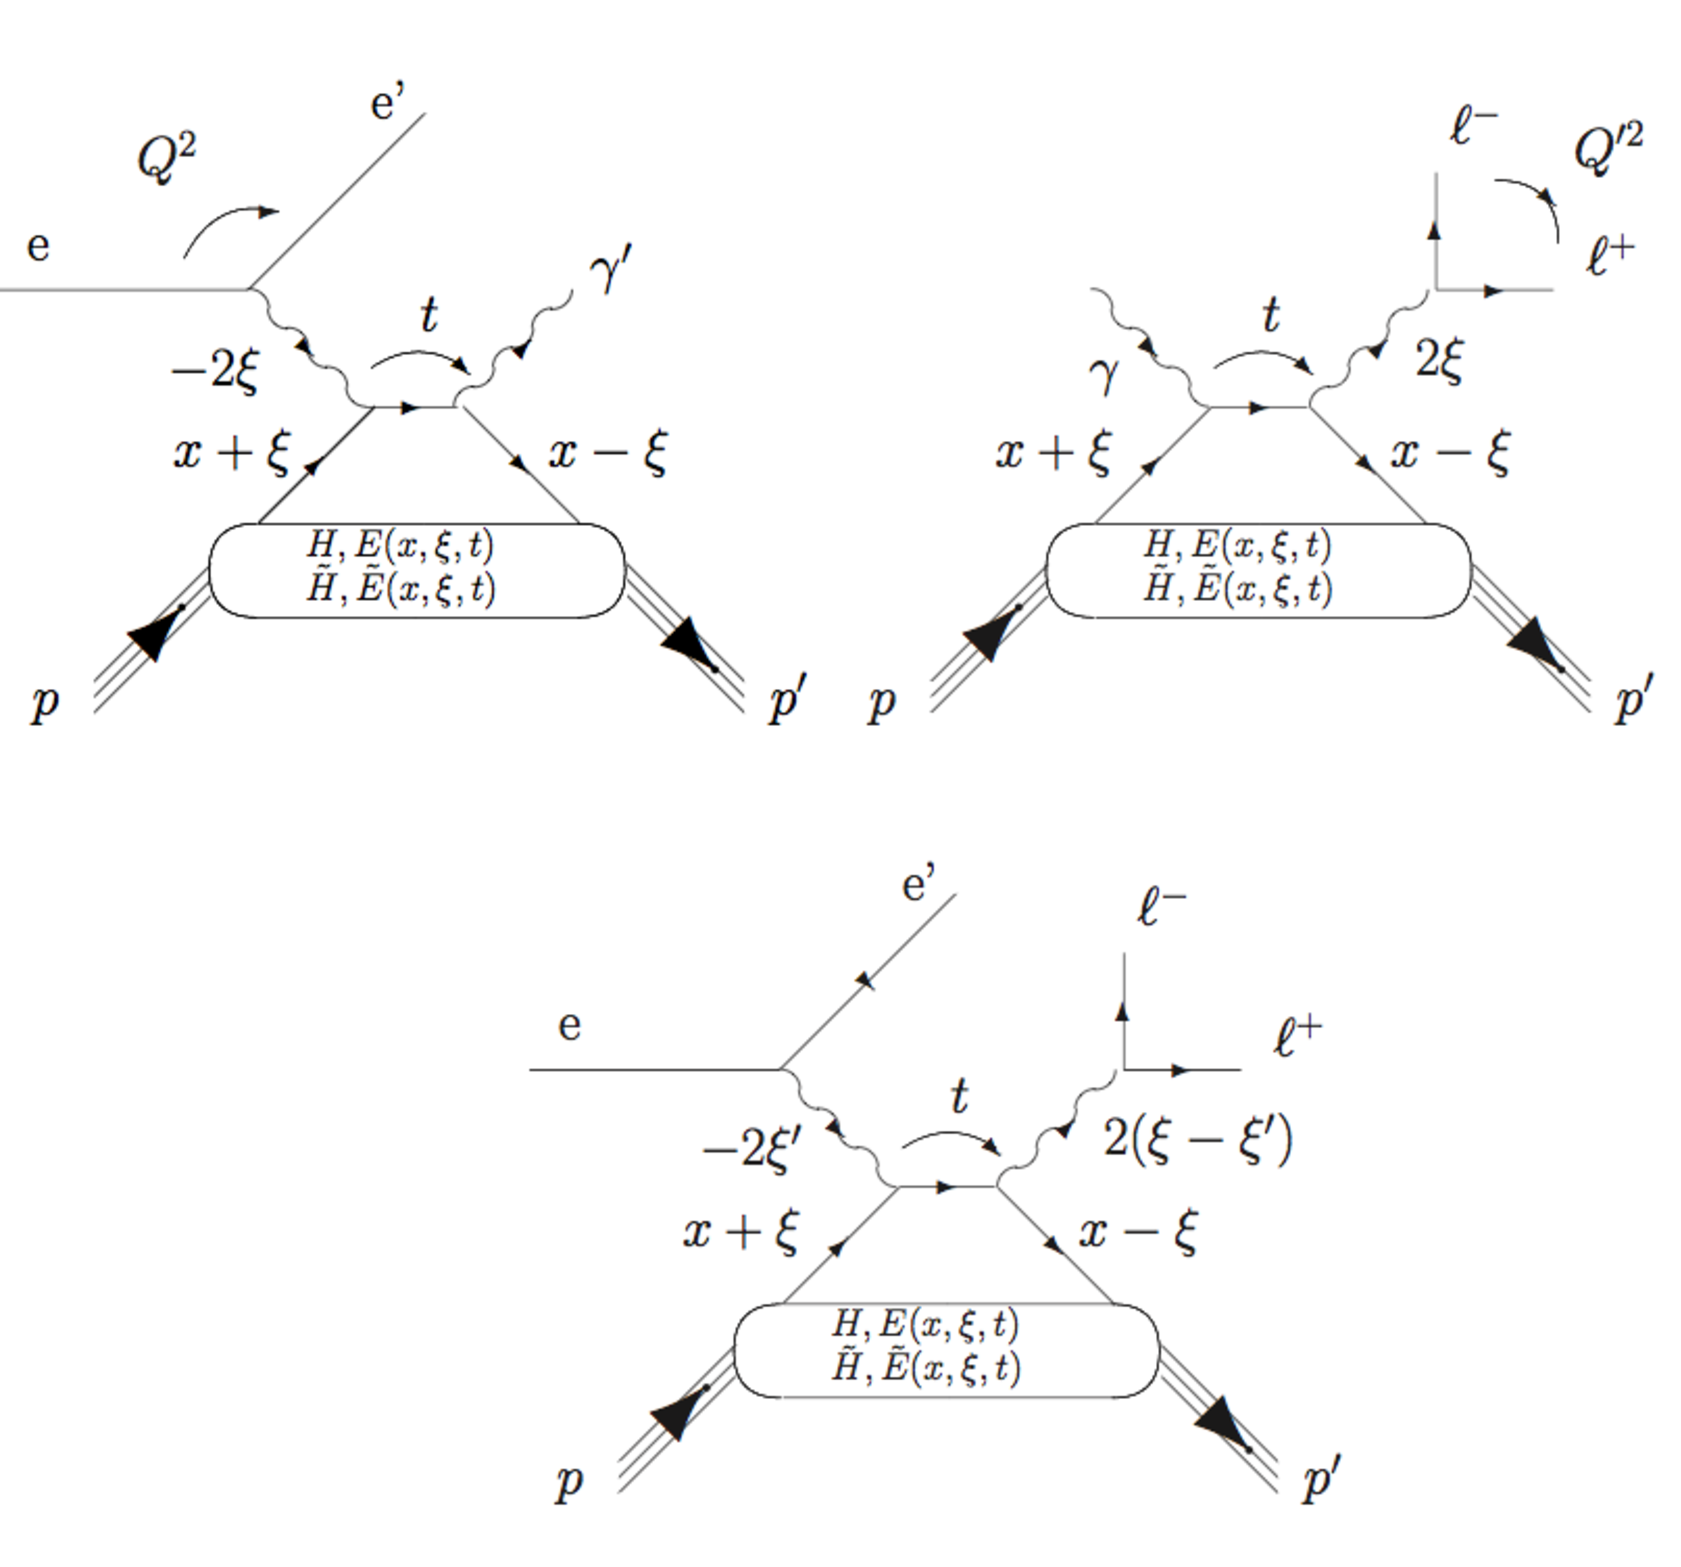
\includegraphics[width=1\textwidth]{3proc.pdf}
\end{center}
\caption{Top left: DVCS handbag diagram. Top right: TCS handbag diagram.
Bottom: DDVCS handbag diagram. Only ``direct" diagrams are shown. There are
also ``crossed" diagrams. In a frame where the nucleon
moves at the speed of light along a certain direction, the longitudinal 
momentum fractions of the particles are also indicated.}
\label{fig:diags}
\end{figure}

There are, at leading twist QCD, four GPDs, called
$H, \tilde H, E, \tilde E$ which reflect the four independent
quark-nucleon helicity-spin transitions between the initial
and final states. They depend upon three variables~: 
$x$, $\xi$ and $t$. As illustrated in Fig.~\ref{fig:diags},
$x+\xi$ is the {\it longitudinal} momentum fraction carried by 
the initial quark struck by the spacelike virtual photon and $x-\xi$ is 
{\it longitudinal} momentum fraction carried by the final quark going 
back in the nucleon after radiating a photon. In Ji's notation~\cite{Ji:1996nm},
the variable varies $x$ between $-1$ and $1$ while the variable $\xi$ 
varies between $0$ and $1$ (due to time reversal invariance, the range of $\xi$ 
can be reduced to this range). One way to interpret the GPDs is therefore as
the probability amplitude of finding a quark (if $|x| > \xi$, or an antiquark 
if $x<-\xi$) in the nucleon with a longitudinal momentum fraction $x+\xi$
and of putting it back into the nucleon with a longitudinal momentum
fraction $x-\xi$ plus some transverse momentum ``kick", which is
represented by $t$. One notes the interesting region $ -\xi < x < \xi$ 
where one ``leg" in Fig.~\ref{fig:diags} 
has a positive momentum fraction (a quark) while the other one has a negative one
(an antiquark). In this region, GPDs behave like a meson distribution amplitude
and can be interpreted as the probability amplitude of finding 
a quark-antiquark pair in the nucleon. 
At $\xi=0$, $t$ can be interpreted as the conjugate variable of the
{\it transverse} impact parameter $b_\perp$ and GPDs describe then the probability 
amplitude of finding in a nucleon a parton with a {\it longitudinal} momentum 
fraction $x$ at a given {\it transverse} distance $b_\perp$ from the
center of the nucleon.

\begin{figure}[htbp]
%\begin{minipage}[t]{76mm}
\begin{center}
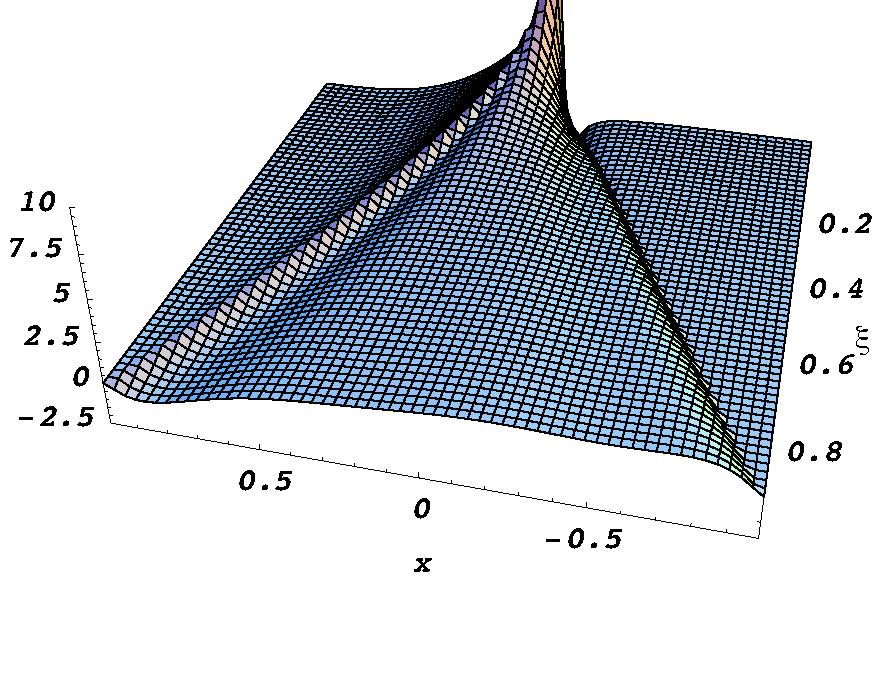
\includegraphics[width=0.7\textwidth]{gpdxxi.pdf}
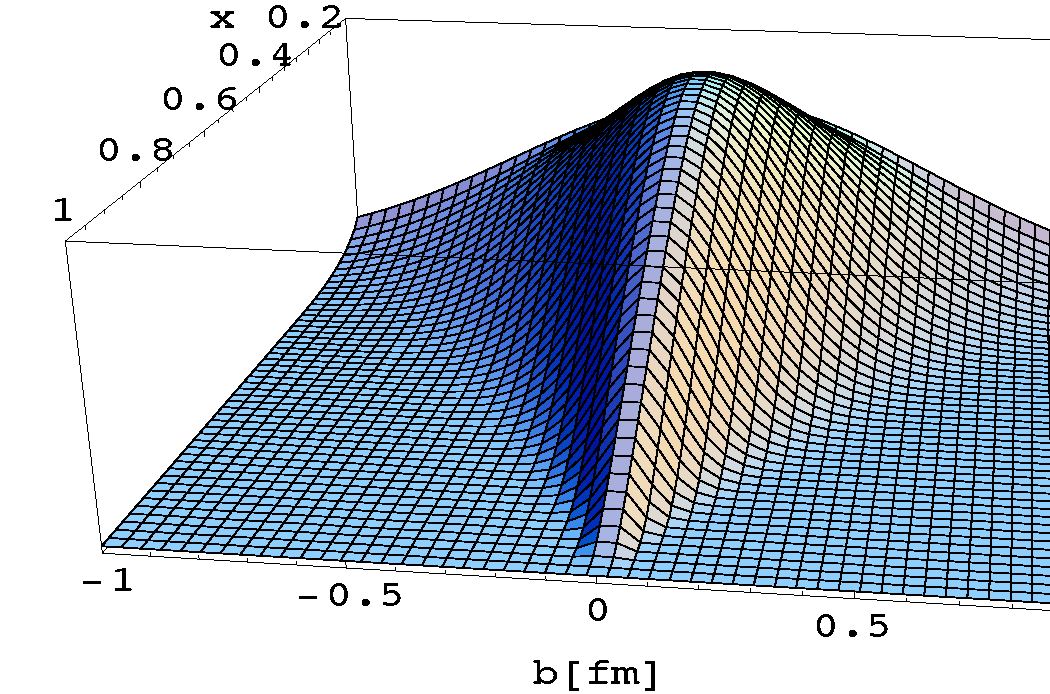
\includegraphics[width=0.7\textwidth]{gpdb_h_u_new.pdf}
%\end{minipage}
%\vspace{-2cm}
\caption{Top: the GPD $H^u(x,\xi,t)$ as a function of the 
{\it longitudinal} momentum fraction $x$ and the {\it longitudinal} 
momentum transfer $\xi$ at $t=0$ according to the VGG model.
One recognizes for $\xi$=0 the typical shape of a parton distribution (with 
the sea quarks rising as $x$ goes to 0, the negative $x$ part being interpreted 
as the antiquark contribution) and as $\xi$ increases the (asymptotic) shape of
a distribution amplitude. Bottom: the GPD $H^u(x,\xi,t)$ as 
a function of the {\it longitudinal} momentum fraction $x$ and 
the {\it transverse} impact parameter $b_\perp$ (the conjugate variable of $t$)
at $\xi=0$ according to the VGG model}
\label{fig:gpdxxi-bperp}
\end{center}
\end{figure}

Fig.~\ref{fig:gpdxxi-bperp} shows, according to one patricular 
GPD model (VGG~\cite{marcprl2,goeke}),
how the ($x$,$\xi$) and the ($x$,$b_\perp$) correlations could look like.
It shows the richness and novelty of the GPDs: information on
$q{\bar q}$ configurations in the nucleon, correlations between quarks 
(or antiquarks) of different momenta, correlations between longitudinal
momentum and trsanverse position of partons (nucleon ``tomography").

We have just seen a crucial issue in the GPD formalism is that the GPDs 
depend on three variables~: $x$, $\xi$ and $t$, but only two of these 
three variables are accessible experimentally, $\xi$ and $t$.
In DVCS, $\xi$ is approximated as $\xi=\frac{x_B}{2-x_B}$, fully
defined by detecting the scattered lepton, and in TCS, $\xi$
is approximateded as $\xi=\frac{Q'^2}{2s-Q'^2}$, fully defined by 
detecting the final leptons.% (all at given beam energies).

The squared momentum transfer $t$ is defined both in DVCS and in TCS by 
detecting either the recoil proton or the outgoing photon.
The variable $x$ is however integrated over in both the DVCS and TCS
amplitudes, due to the loop in the ``handbag" diagrams (see Fig.~\ref{fig:diags}).
Precisely, the DVCS amplitude is proportional to:
\begin{eqnarray}
\int_{-1}^{+1}d x {{H(x,\xi,t)} \over {x - \xi + i \epsilon}}+...
\end{eqnarray}
(where the ellipsis stand for similar terms in $E$, $\tilde{H}$
and $\tilde{E}$). 
The ${1} \over {x - \xi + i \epsilon}$ term is the propagator of the quark 
between the incoming virtual photon and the outgoing photon.
The previous expression can be decomposed into a real and an imaginary parts:
\begin{eqnarray}
PV(\int_{-1}^{+1}d x {H(x,\xi,t) \over {x - \xi}})-i\pi H(\xi,\xi,t)
\end{eqnarray}
This means that the maximum information that can be extracted from the experimental 
data at a given ($\xi,t$) point is $H(\pm\xi,\xi,t)$, when measuring an observable
particularly sensitive to the imaginary part of the DVCS amplitude (such as single beam 
or target spin asymmetries), and $\int_{-1}^{+1}d x {H(\mp x,\xi,t) 
\over {x \pm \xi}}$, when measuring an observable particularly
sensitive to the real part of the DVCS amplitude (such as unpolarized
cross sections or double-spin beam/target spin asymmetries).

Experimentally, DVCS is accessed by measuring the reaction $ep\to e p\gamma$
and TCS by measuring the reaction $\gamma p\to p \ell^+\ell^-$. However,
DVCS and TCS are not the only processes leading to these final states. There
are also the so-called Bethe-Heitler (BH) processes. In the $ep\to e p\gamma$ reaction,
the BH produces a final state photon which is radiated either
from the incoming or the scattered electron and in the $\gamma p\to p \ell^+\ell^-$,
the final lepton pair originates from the photon beam (see Fig.~\ref{fig:allbh}). 
In both cases, the final state photon (be it real or virtual) doesn't originate
from the nucleon and therefore does not carry any partonic or GPD information.
The BH interferes with DVCS (and TCS) at the amplitude level and
therefore complicates the extraction of the DVCS and TCS (i.e. GPDs) information.
However, it is rather precisely calculable theoretically and can be put
under control.

\begin{figure}[htbp]
\begin{center}
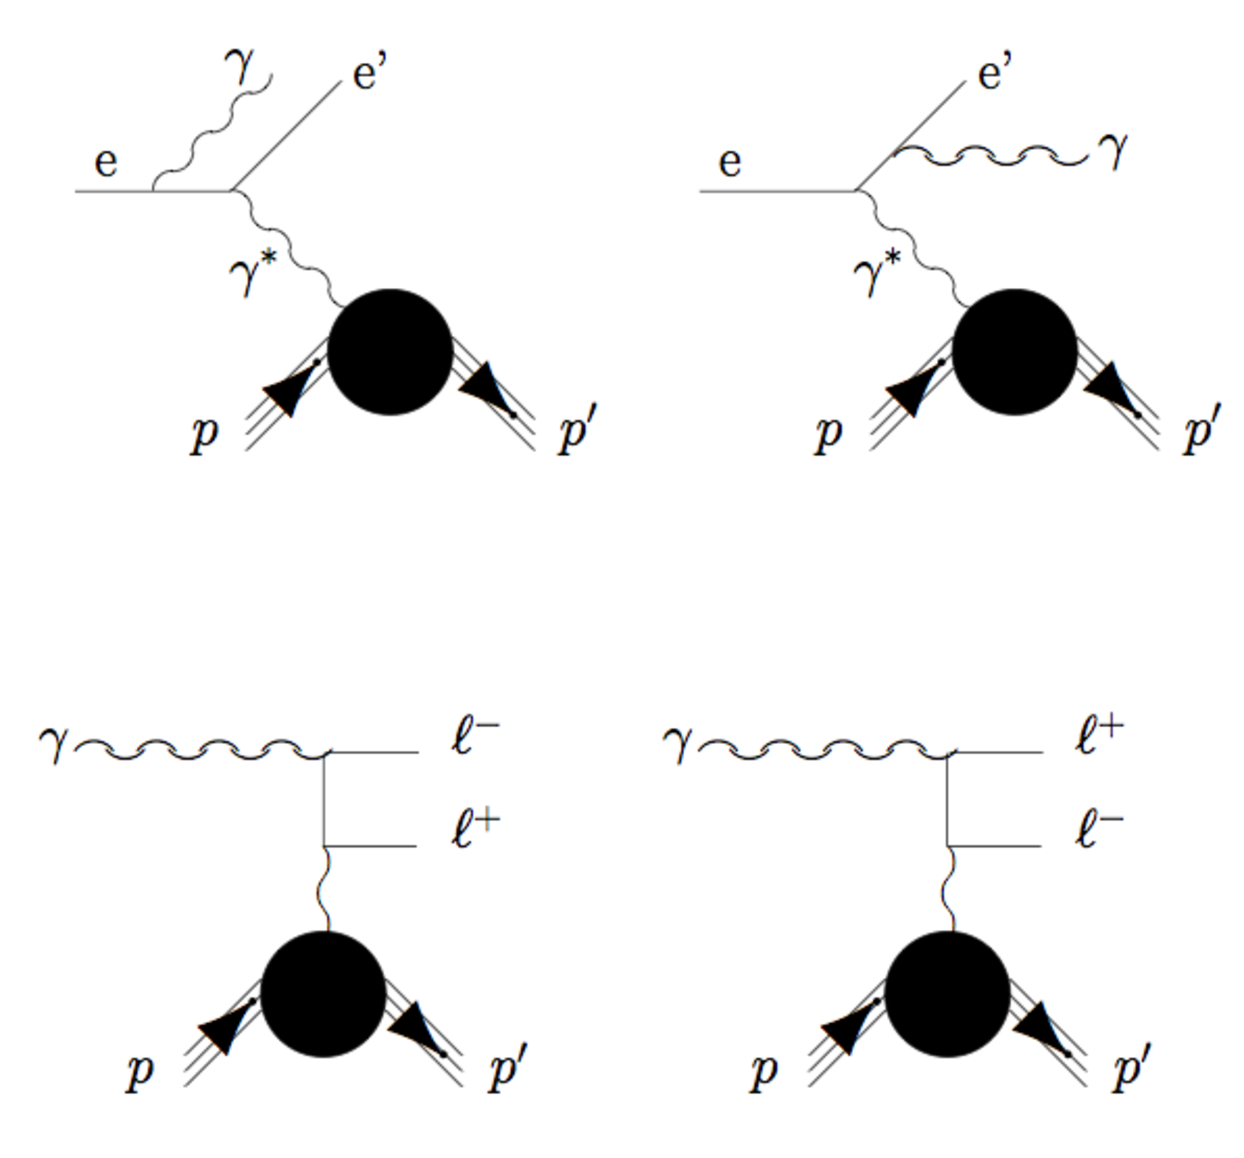
\includegraphics[width=0.8\textwidth]{allbh.pdf}
\end{center}
\caption{Top: the BH diagrams for DVCS. Bottom: the BH diagrams for TCS.
In DDVCS, all four contributions are present (the DVCS-BH diagrams have to
be ``completed" by the decay into a lepton pair of the final state photon 
and in the TCS-BH diagrams, the initial state real photon must
emerge from an electron beam).}
\label{fig:allbh}
\end{figure}

While no experimental data have been published related to TCS (and DDVCS), quite
some data has already been released related to DVCS (on the proton). 
Limiting ourselves to the valence (JLab) region, unpolarized cross 
sections~\cite{carlos,Jo:2015ema}, beam spin asymmetries~\cite{fx} and 
longitudinally polarized target spin asymmetries~\cite{shifeng,erin,Pisano:2015iqa}
(as well as double spin beam-target asymmetries) have been measured. 

These past few years, several groups~\cite{fitmuller,herve,fitmick,fithermes,fittsa,fitall} 
have developped fitting codes and algorithms aimed at extracting the GPD information 
from these DVCS data. We recall the complexity of the task due to,
in particular, the BH contribution in addition to DVCS. These fitting algorithms have 
nevertheless succeeded in extracting
the quantities $H(\pm\xi,\xi,t)$ and $\tilde{H(\pm\xi,\xi,t)}$ at the $\approx 30$\% level
for different values of $\xi$ and $t$ (see Ref.~\cite{rpp} for a compilation of the
fit results). Although the  information thus obtained is already very valuable 
and provides first constraints on GPD models, it is very desirable to extract
the quantities where the first two arguments of the GPDs, $x$ and $\xi$,
are decoupled (i.e. $x\neq\xi$). For instance, ``nucleon imaging"
requires the knowledge of $H(\xi,0,t)$ (and ` for the
other GPDs). With results from DVCS (and TCS) alone, this is not possible.

The way to avoid the $x$-integration issue is DDVCS. Compared to DVCS,
DDVCS contains an additional kinematic lever arm with the timelike virtuality of the
final photon which can can now be varied (by measuring the invariant mass of the
decay leptons pair).
Fig.~\ref{fig:diags} illustrates this where the {\it plus}-components 
(in light-cone kinematics) of
the longitudinal momentum fraction of the quarks and photons are
indicated. In the DDVCS case, the kinematics of the 2 photons 
(incoming and outgoing) is described by 2 variables, $\xi$ and 
$\xi^\prime$, which can be independently varied (whereas, in DVCS,
only $\xi$ can be varied). For DDVCs, there are two diagrams
(only the ``direct" one is shown in Fig.~\ref{fig:diags}) and
their propagators read:

\begin{equation}
{1 \over {x - (2\xi^\prime-\xi) + i \epsilon}} + 
{1 \over {x + (2\xi^\prime-\xi) - i \epsilon}}
\label{eq:ddvcs}
\end{equation}

Therefore, the DDVCS amplitude is proportional to: 
\begin{equation}
\int_{-1}^{+1}d x {{H(x,\xi,t)} \over {x - (2\xi^\prime-\xi) + i \epsilon}}+...
\label{eq:ddvcs2}
\end{equation}

Then, by measuring an observable proportional to the imaginary part of the 
DDVCS amplitude (for instance, the beam asymmetry, like in the DVCS case),
one has access, in a concise notation, to $H(2\xi^\prime-\xi,\xi,t)
+H(-(2\xi^\prime-\xi),\xi,t)$ (keeping the contribution of the crossed term
of Eq.~\ref{eq:ddvcs}.
We refer the reader to Refs.~\cite{Guidal:2002kt,ddvcs_bm1,ddvcs_bm2} 
for the details of the formalism. This therefore allows for maping the GPD's along each
of the three axis ($x$, $\xi$ and $t$) as the three variables can now 
be varied independently. 

Experimentally, $\xi^\prime=\frac{x_B}{2-x_B}$,
i.e. it is fully defined by the detection of the scattered electron,
and $\xi=\xi^\prime\frac{Q^2+Q'^2}{Q^2}$, i.e. it requires 
in addition the determination of the (squared) invariant mass of the lepton
pair $Q'^2$. In other words, if one fixes $x_B$, one defines uniquely $\xi^\prime$
and if one fixes $Q^2$ and $Q'^2$ according to the combination in the
previous sentence, one defines uniquely $\xi$. In order
to access the combination $H(2\xi^\prime-\xi,\xi,t)+H(-(2\xi^\prime-\xi),\xi,t)$,
one should thus aim at measuring the DDVCS beam asymmetry at fixed $x_B$,
$Q^2$ and $t$ for a series of $Q'^2$ values (one can actually also vary $Q^2$,
as long as the combination $\frac{Q^2+Q'^2}{Q^2}$ remains constant
so as to keep $2\xi^\prime-\xi$ fixed).

Fig.~\ref{fig:asym_ddvcs} shows for instance the predicted beam spin asymmetries
for the DDVCS process at typical JLab beam energies for different $Q'^2$
values. We recall that this asymmetry arises
from the interference between the DDVCS and the associated Bethe-Heitler 
processes, which are a generalization of the four diagrams of Fig.~\ref{fig:allbh} 
(the final state real photon of the ``DVCS-BH" diagrams is to decay
into a lepton pair and the initial state real photon of the ``TCS-BH" diagrams
is to be radiated from an electron beam). One recognizes the familiar
sinus-like shapes as a function of $\phi$, the azimutal angle
between the leptonic and hadronic planes.
We also recall that only $Q'^2=0$ can be accessed in DVCS.
The dependence on $Q'^2$ reflects the variation of the first argument
of the GPD ($x=2\xi^\prime-\xi$) for a given second argument $\xi$ (i.e. $x_B$).
Fig.~\ref{fig:asym_ddvcs} shows that there is a strong sensitivity 
which should ultimately allow the extraction of the GPDs in the $(x,\xi)$ plane.

\begin{figure}[htbp]
\begin{center} 
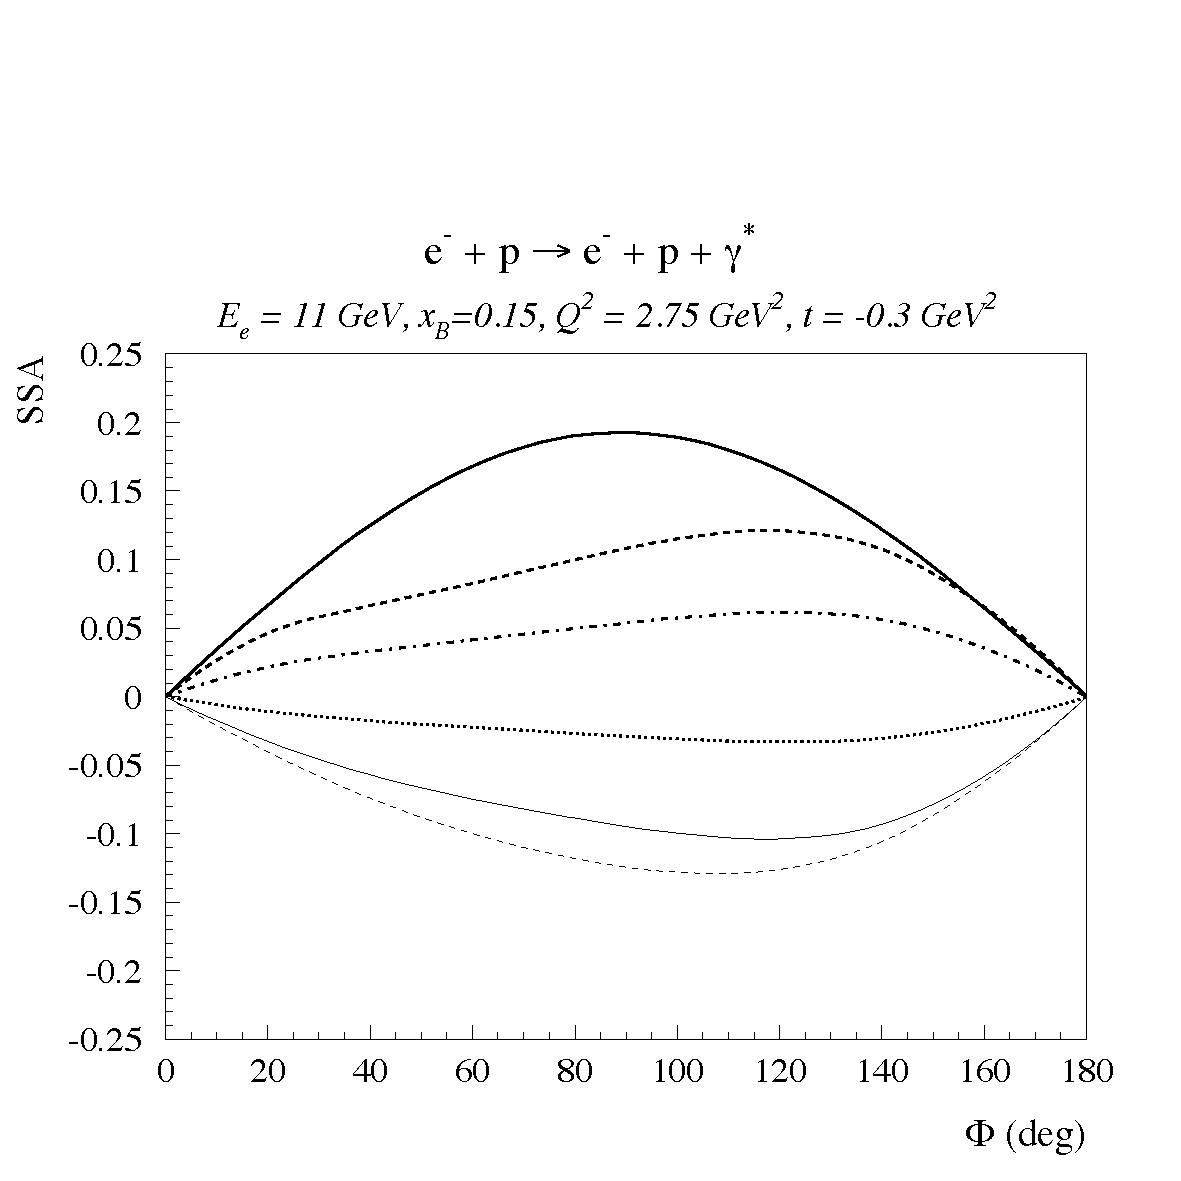
\includegraphics[width=1\textwidth]{asymm_ddvcs.pdf}
\caption{Beam spin asymmetry for the reaction $ep\to e^\prime p\mu^+\mu^-$ (DDVCS+BH) 
for different virtualities of the lepton pair~:
$Q'^2$ = 0. (thick solid line), 1.5 (thick dashed line), 2. (thick dash-dotted line), 2.8 (dotted line)
3.6 (thin solid line) and 4.4 GeV$^2$ (thin dashed line). Calculations and predictions 
from~\cite{Guidal:2002kt}. The kinematics has been integrated over the
2 decay angles.}
\label{fig:asym_ddvcs}
\end{center}
\end{figure}

In Fig.~\ref{fig:asym_ddvcs}, it is very interesting to note the change
in sign of the beam spin asymmetry as one goes from the region $Q'^2<Q^2$
to the region $Q'^2>Q^2$. it can be said that one goes from the
``spacelike-dominated" region to the ``timelike-dominated" region,
or from the ``DVCS-dominated" region to the ``TCS-dominated" region.
It was shown in Ref.~\cite{Muller:2012yq} that the TCS amplitude is the conjugate
of the DVCS amplitude. One can therefore understand the change in
sign of the beam spin asymmetry in Fig.~\ref{fig:asym_ddvcs} as one crosses 
the $Q^2=Q'^2$ region as a change in sign of the imaginary
part of the DDVCS amplitude. This is a prediction of the ``handbag"
formalism and a very strong test that one is in the right regime
to access GPDs. One should note that the region around $Q'^2=Q^2$
might not directly applicable to the GPD formalism. Indeed, in this
region, the quark in the propagator of the DDVCS diagram in Fig.~\ref{fig:diags}
has a momentum close to 0 as $Q'^2=Q^2$ is essentially equivalent
to $2\xi^\prime-\xi=0$. Therefore, pQCD factorization will break down
and soft scales and mechanisms will enter into play. Even though this
particular region $Q'^2=Q^2$ might not be directly interpretable
in terms of GPDs, it should clearly be extremely interesting to
make measurements at those kinematics to understand the transition
between soft and hard mechanisms.

\begin{figure}[htbp]
\begin{center} 
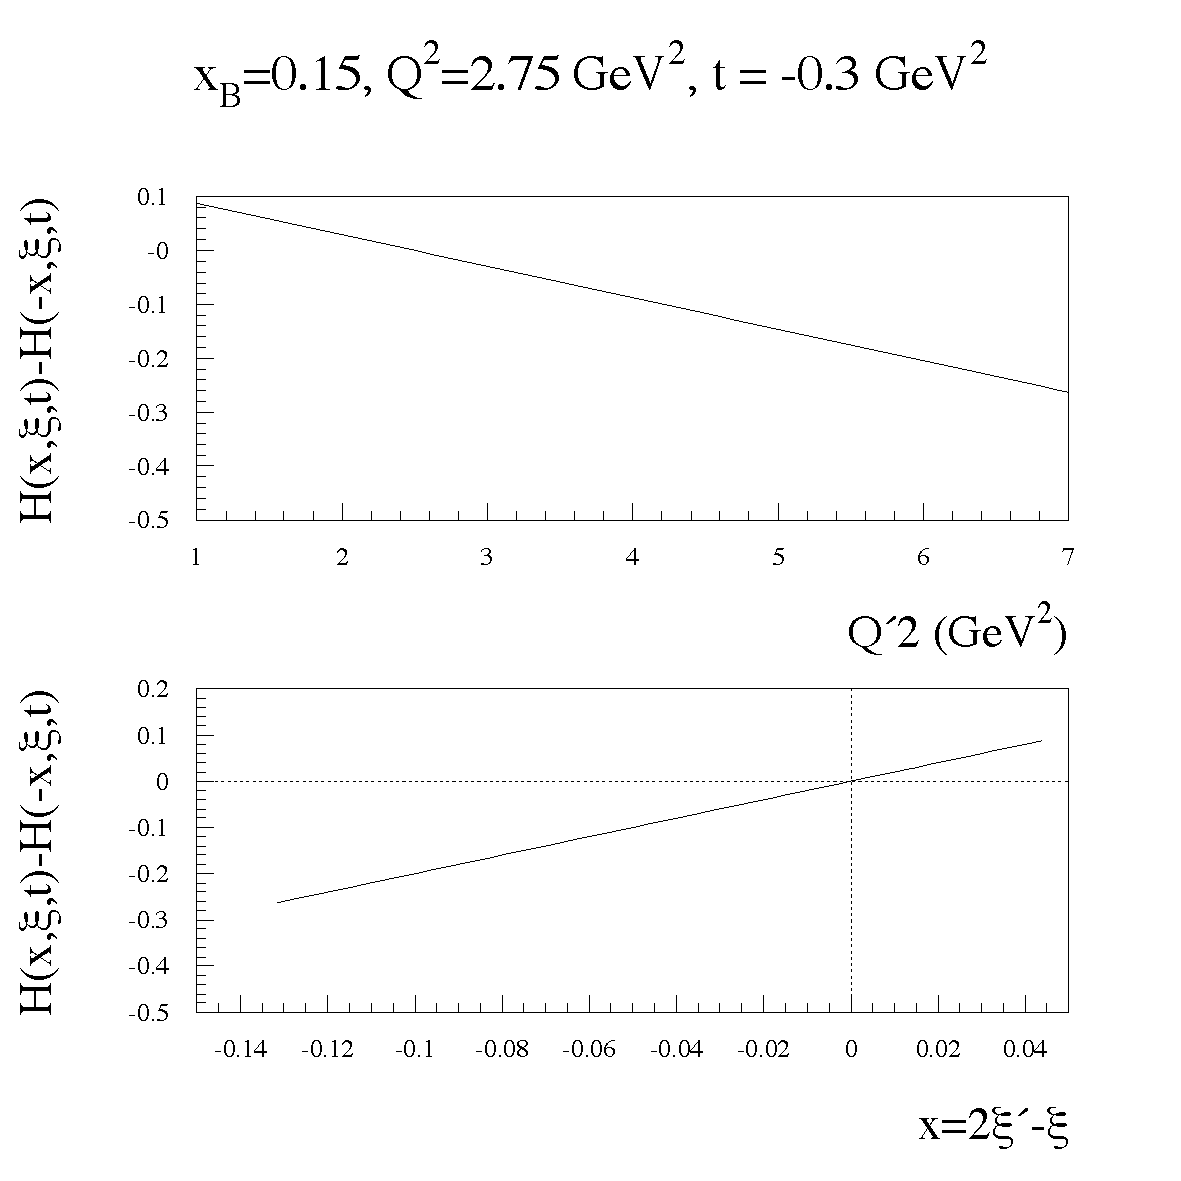
\includegraphics[width=1\textwidth]{scan_ddvcs.pdf}
\caption[]{Assuming the dominance of the $H$ GPD in the DDVCS beam spin asymmetry,
the GPD combination $H(2\xi^\prime-\xi,\xi,t)+H(-(2\xi^\prime-\xi),\xi,t)$
that can be accessed, as a function of $Q'^2$ (top panel)
or equivalently $2\xi^\prime-\xi$ (bottom panel), for fixed $\xi^\prime$ (i.e.
$x_B$) and fixed $t$. In the bottom panel, the negative $2\xi^\prime-\xi$
region allows to access the $-(H(2\xi^\prime-\xi,\xi,t)+H(-(2\xi^\prime-\xi),\xi,t))$
GPD combination for positive $2\xi^\prime-\xi$, due to the symmetry of the
problem.}
\label{scan-ddvcs}
\end{center}
\end{figure}

In Fig.~\ref{scan-ddvcs}, we show the range in $2\xi^\prime-\xi$
that can be accessed at the particular kinematics: $E_e$=11 GeV,
$x_B$=0.15 (i.e. $\xi\approx$0.8), $Q^2$=2.75 GeV$^2$ and $-t$=0.3 GeV$^2$,
by varyong $Q^2$ from 1 to 7 GeV$^2$. One notes in particular
the (anti-)symmetry around $2\xi^\prime-\xi$ which reflects the
quasi (anti-)symmetric behavior of the beam spin asymmetry of
Fig.~\ref{asym-ddvcs} around $Q^2=Q'^2$. One has therefore
two relatievly independent ways of measuring the same
combination of GPDs $H(2\xi^\prime-\xi,\xi,t)+H(-(2\xi^\prime-\xi),\xi,t)$:
in the region $Q^2<Q'^2$ and in the region $Q^2>Q'^2$. Only the sign
of the combination varies as one amplitude is the conjugate of the other.

Of course, the downside of the DDVCS process is however the very low cross section
involved. Indeed, due mainly to the extra $\alpha_e\approx 1/137$ coupling
introduced by the decay of the outgoing photon into the lepton pair,
the cross section is about a factor 300~\cite{Guidal:2002kt} less than the
DVCS process, at $Q'^2\approx .3$ GeV$^2$ for instance. 

We recall that the beam spin asymmetry for DVCS has been measured~\cite{fx}
for $\approx$ 20 ($x_B$, $Q^2$, $t$) bins with the JLab 6 GeV beam 
and the CLAS detector with a luminosity of 10$^{34}$cm$^{-2}$s$^{-1}$.
As we will be shown in the following of this document, it is anticipated
to run with the JLab 12 GeV beam and the CLAS12 detector at a luminosity
of 10$^{37}$cm$^{-2}$s$^{-1}$. Intuitively, it can therefore be anticipated
that the DDVCS beam spin asymmetry measurement should be feasible,
taking also into account an extra factor for the final state lepton pair
detection efficiency.

%\end{document}

\clearpage

\subsection{J/$\Psi$ Electroproduction}
N. Baltzel, F-X. Girod, S. Stepanyan

The proposed $e\mu^+\mu^-$ final state will contain events from the $J/\psi$ electroproduction. measure the cross section of $J/\psi$ photoproduction 
on the proton near threshold ($E_{\gamma, {\rm threshold}} = 8.21$ GeV).

$J/\psi$ production near threshold is a rich and complex physics 
topic in its own right and presently the subject of intense theoretical 
research. The measurement of the $J/\psi$
photoproduction cross section is of great interest for the purpose of a
precise yield extraction. The projected results would, however, represent
a dramatic improvement over the world data on $J/\psi$ production near
threshold, and would thus impact the on-going theoretical discussions.
In this section we briefly describe the current understanding of 
$J/\psi$ production near threshold, the projected results, and the
role of the $J/\psi$ measurement in the present DDVCS experiment.


\subsection{$J/\psi$ production near threshold}
\label{subsec:JPsi}

The production of heavy quarkonia and their interaction with hadronic
matter are key questions of QCD, which are being studied through 
production experiments at different energies and various theoretical 
approaches; see Ref.~\cite{Brambilla:2010cs} for a recent review. 
Because of the small spatial size of heavy quarkonia on the hadronic 
scale, $r_{Q\bar Q} \ll 1~{\rm fm}$, one can use QCD operator methods
to describe their interactions with hadrons and external probes in
controlled approximation. Heavy quarkonium production probes the local 
color (gluon) fields in the nucleon, and can reveal properties such as 
their response to momentum transfer, their spatial distribution,
and their correlation with valence quarks. The dynamics that produces
the relevant gluon fields in the nucleon changes considerably
between high energies and the near-threshold region, creating a fascinating
landscape that calls for detailed experimental study. At high energies
($W > 10 \, {\rm GeV}$) exclusive $J/\psi$ photo-- and electroproduction 
probes the nucleon's gluon GPD at small momentum fractions 
$x \sim M_{J/\psi}^2/W^2 \ll 1$ and can be used to infer the transverse 
spatial distribution of small--$x$ gluons in the nucleon; 
see Ref.~\cite{frankfurt:2005mc} for a review; such experiments were 
performed at HERA \cite{aktas:2005xu,chekanov:2004mw} and FNAL 
\cite{binkley:1981kv}, and a detailed program of ``gluon imaging'' 
along these lines is planned with a future Electron Ion 
Collider (EIC) \cite{Boer:2011fh}. In exclusive $J/\psi$ production 
near threshold, the minimum invariant momentum transfer to the nucleon 
becomes large: $|t_{\rm min}| = 2.23$ GeV$^2$ at threshold, 
and $|t_{\rm min}| = 1.3-0.4$ GeV$^2$ in the $E_{\gamma} = 8.5-11$ 
GeV range. The process is therefore analogous to elastic $eN$ scattering 
at large $|t|$, only that the ``probe'' couples to the gluon field 
in the target. Exclusive $J/\psi$ production near threshold thus 
measures the nucleon form factor of a gluonic operator and can provide
unique information on the non-perturbative gluon fields in the nucleon.

The precise identification of the gluonic operators associated with
$J/\psi$ production near threshold and the modeling of their nucleon
form factors are the subject of intense theoretical research, the
status and perspectives of which were summarized at a recent topical
workshop \cite{temple}. Several approaches are presently being discussed. 
One scenario assumes that even near threshold the $J/\psi$ is produced 
through two--gluon exchange with a GPD--like coupling to 
the nucleon, but now in the special kinematics of large 
$|t| \sim |t_{\rm min}|$ and large ``skewness'' 
$\xi \sim 0.5$ \cite{frankfurt:2002ka}. A more likely possibility
is that the production process near threshold effectively reduces to 
a local gluonic operator, implying simple kinematic scaling 
relations~\cite{weiss:temple}. Another scenario uses the hard scattering 
mechanism for high-$t$ elastic form factors and assumes that the 
production process happens in the leading 3-quark 
Fock component of the nucleon, with rescattering through hard
gluon exchange~\cite{brodsky:2000zc}. $J/psi$ production near threshold 
is also being studied in the non--relativistic QCD (NRQCD) scheme,
which attempts a systematic parametric expansion in the heavy quark 
velocity~\cite{Butenschoen:2009zy,Butenschoen:2011yh}; first results 
for JLab 12 GeV kinematics were reported 
in Ref.~\cite{Butenschoen:temple}.

It is clear that progress with unraveling the mechanism of $J/\psi$ 
production near threshold depends crucially on experimental input.
Because of the small cross sections exclusive $J/\psi$ production 
near threshold was never measured with the precision necessary to 
discriminate between the proposed dynamical scenarios, let alone to 
extract quantitative information on the relevant operators probing 
the color fields in the nucleon. The existing data from the SLAC
and Cornell experiments~\cite{gittelman:1975ix,camerini:1975cy}
(see Fig.~\ref{fig:jpsixs}) provide some rough information on 
the energy dependence of the exclusive photoproduction cross section
and the $t$--slope near threshold. The present CLAS12 experiment
represents a unique opportunity to explore the unmeasured 
near--threshold region from $E_{\gamma} \approx 8.5 \, \textrm{GeV}$
to $11 \, \textrm{GeV}$. The projected data would dramatically
extend and improve our knowledge of the $J/\psi$ photoproduction
cross section and $t$--dependence near threshold (see Sect. \ref{sec:jprate}),
and directly impact on the on--going theoretical studies of the
reaction mechanism.


\subsection{Impact on the DDVCS measurement}
\label{sec:jpsi_ddvcs}


Since the final states for DDVCS and J/$\psi$ are identical, the detector efficiency and resolution for exclusive $J/\psi$
production is very similar to that of DDVCS events in the proposed range of lepton invariant mass. The narrow peak of the $J/\psi$ will make it easy to identify the reaction, and more suitable for a reliable yield extraction than the DDVCS-BH continuum. The $J/\psi$ electroproduction
reaction can thus serve as an important benchmark, allowing us to better
understand the systematic uncertainties.
The $\phi(1020)$ could in principle also be used in a similar way at the
lower end of the invariant mass range.
A measurement of the $J/\psi$ cross section in parallel with DDVCS will thus
be very beneficial for the understanding the DDVCS data, and help addressing
the two main sources of systematic uncertainty, i.e. acceptance
and the muon identification.
%This is discussed further in Sect.~\ref{sec:systematics}.





\section{The Experiment}
\indent

We propose to study di-muon electroproduction on hydrogen using the CLAS12 detector in experimental Hall-B and the 11 GeV longitudinally polarized electron beam. The reaction - 
\begin{eqnarray}
ep\to e^\prime ~\mu^+ ~\mu^- ~p^\prime
\end{eqnarray}
will be studied in wide range of W, Q$^2$, t, and M$_{\mu\mu}$ (Q$^{\prime 2}$).  
Only the electron and the muon pair in the final state will be detected, the recoil proton will be reconstructed in the missing momentum analysis. For detection and identification of the $e\mu^+\mu^-$ final state the CLAS12 Forward Detector (FD) will be used after some modifications.
For this measurements, the CLAS12 Central detector will not be needed since as it will be shown in Section \ref{acc_simulations} there are no final state particles in the region kinematics of proposed measurements that will be produced in its detection region. But we still intend to use the solenoid magnet for protection of the forward detectors from M\"{o}ller electrons.


\subsection{Detector Configuration}
\indent

\label{detector}
The proposed experiment requires (a) detection of muons and (b) much higher luminosity than CLAS12 design luminosity. The luminosity limit for CLAS12 is mostly defined by the electromagnetic background, in particular from M\"{o}ller electrons flooding the forward drift chambers (FDC). In the nominal configuration, combination of the solenoid field ($\sim$ few Tesla) and the M\"{o}ller cone, a tungsten cone with an opening for the beam that covers region of angles up to $3$ degrees, ensure the acceptable occupancy in FDC at luminosity of $\sim 10^{35}$ cm$^{-2}$ sec$^{-1}$. This proposal aims to run with $\sim 50 ~-~ 100$ times higher luminosity. The detector configuration presented here is designed to provide high luminosity running capability and the detection of muons in the CLAS12 Forward Detector. 

The plane view of the CLAS12 (cut in (YZ) plane) is shown in Fig. \ref{fig:clas12}. As a simple solution, we propose to remove the High Threshold Cherenkov Counter (HTCC) and increase the size of the M\"{o}ller cone (shown in gold) to cover the whole acceptance region of HTCC (shown with red ellipse). In this case the forward drift chambers will be fully protected from any background generated in the target and will be able to handle higher luminosities. With adequate thickness this shielding will be used as absorber for charged hadrons in the muon detector, which is CLAS12 FD. For the detection of the scattered electrons, a compact, highly segmented PbWO$_4$ calorimeter will also be used, which will be part of the shielding.  

\begin{figure}[h]
\centering
%\begin{picture}(80,60)
%\put(-120,-100)
{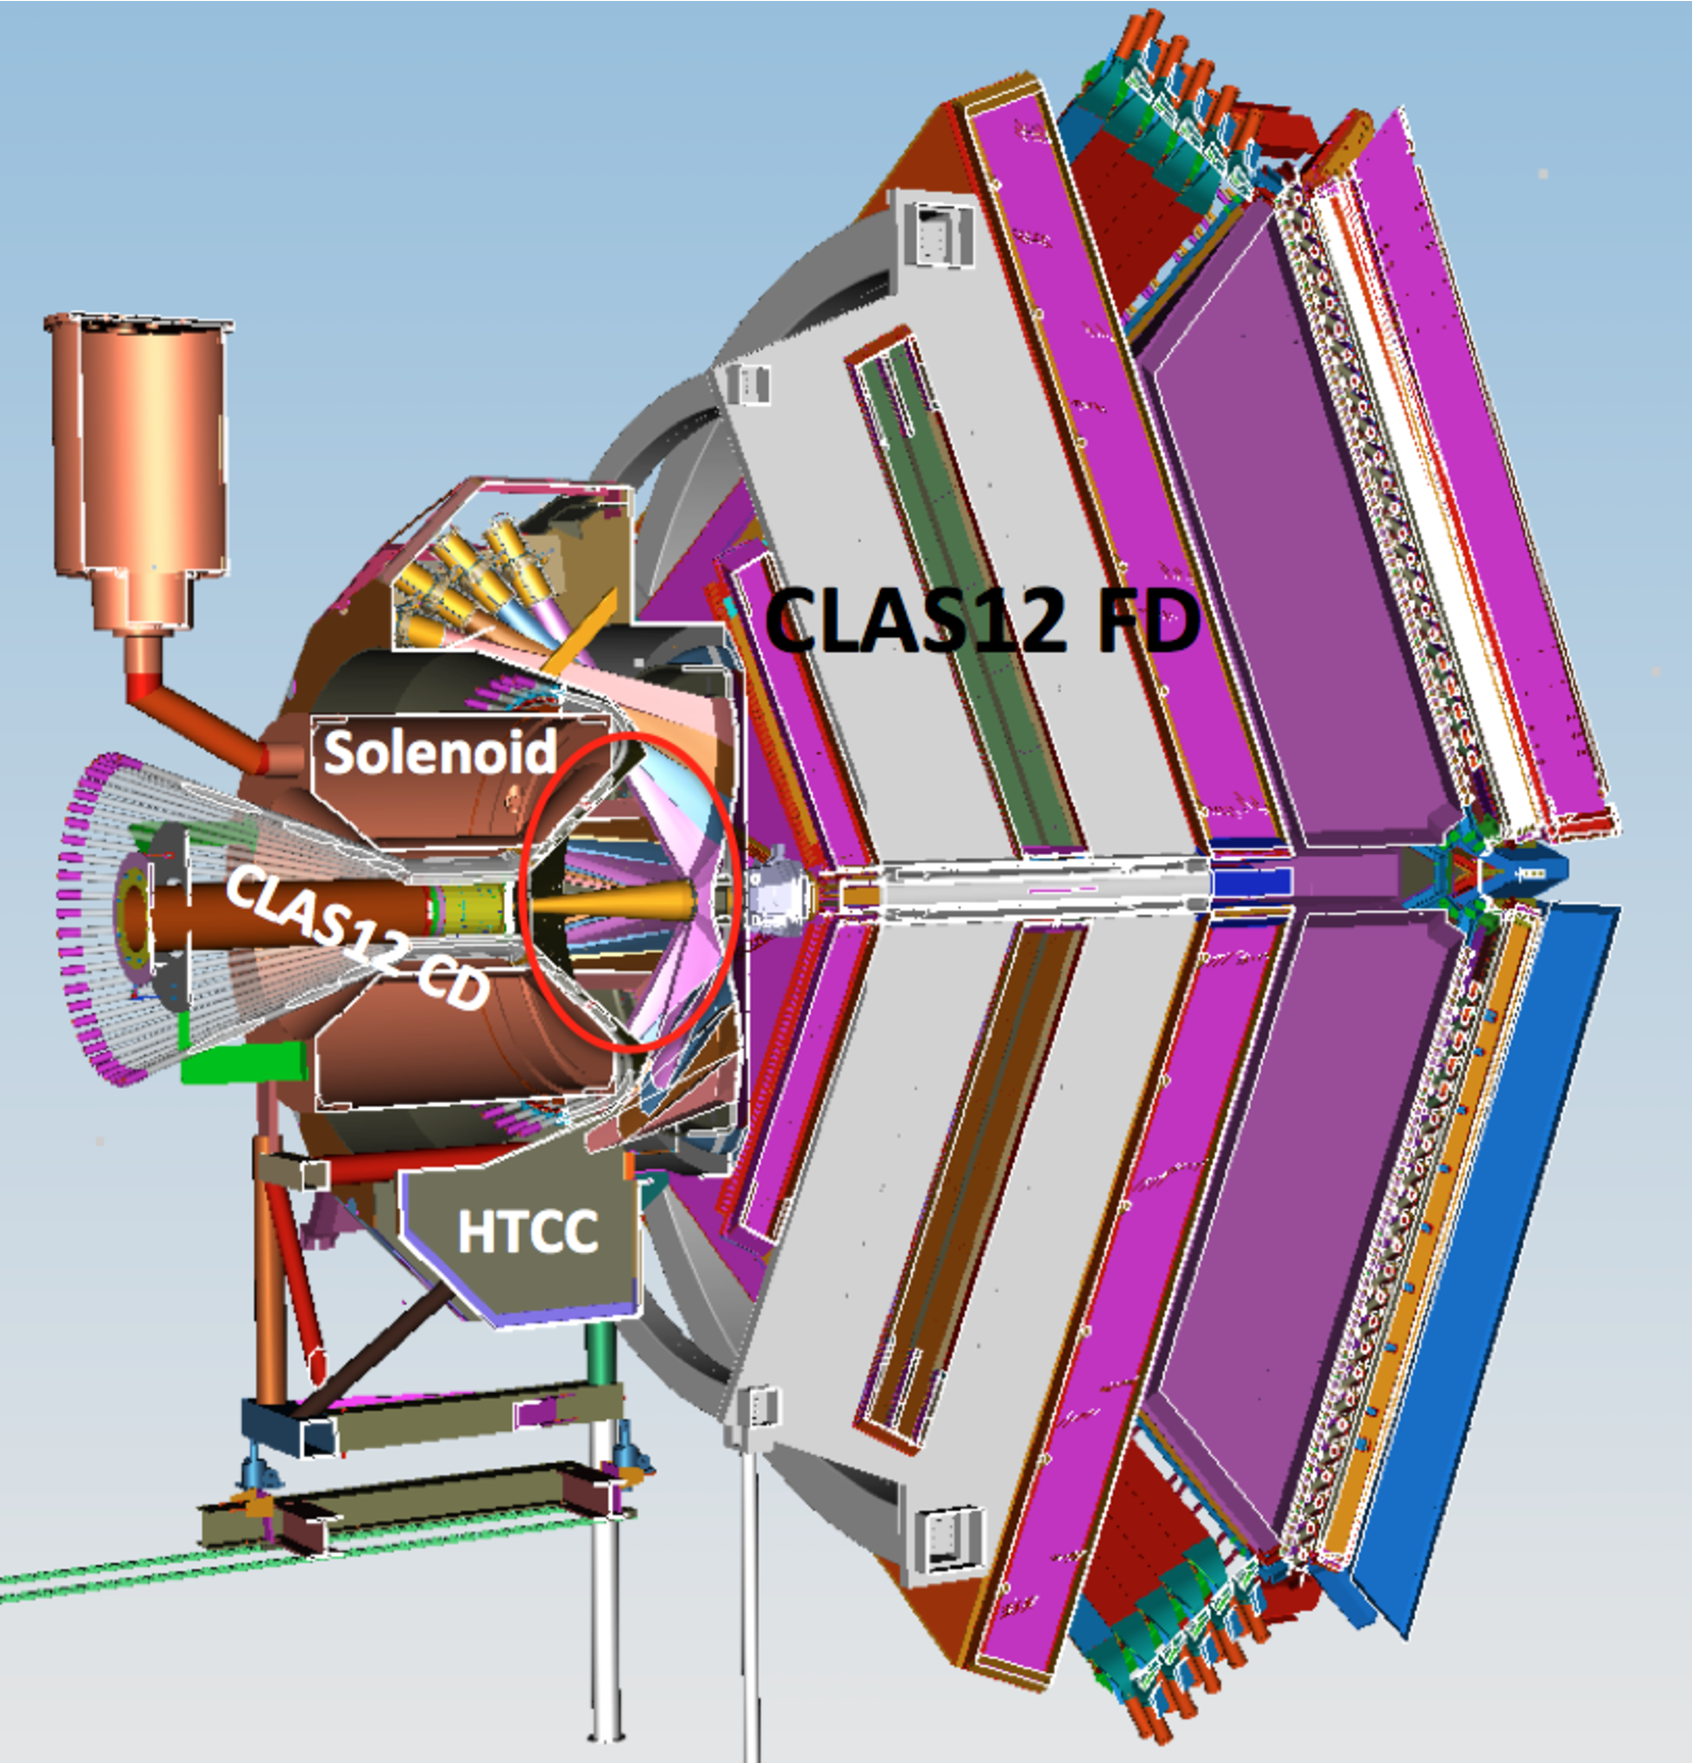
\includegraphics[width=0.9\textwidth]{clas12.pdf}}
%\put(-5,150){Solenoid}
%\end{picture}
\caption{The CLAS12 detector in Hall-B, mid plane cut view. The region of the working volume of HTCC is shown with red contour.}
\label{fig:clas12}
%\end{center}
\end{figure}

A concept of such shielding-calorimeter is shown in Fig. \ref{fig:shield}. The shield is $60$ cm thick and starts at $100$ cm from the target center. It extends to $35$ degrees in polar angle, the full range of the CLAS12 FD. The calorimeter used for the detection of the scattered electrons covers a polar angular range from $5$ to $35$ degree, and has $\pi/3$ in azimuthal coverage. The coverage and granularity of the calorimeter will be optimized with further simulations. 

\begin{figure}[h]
\begin{center}
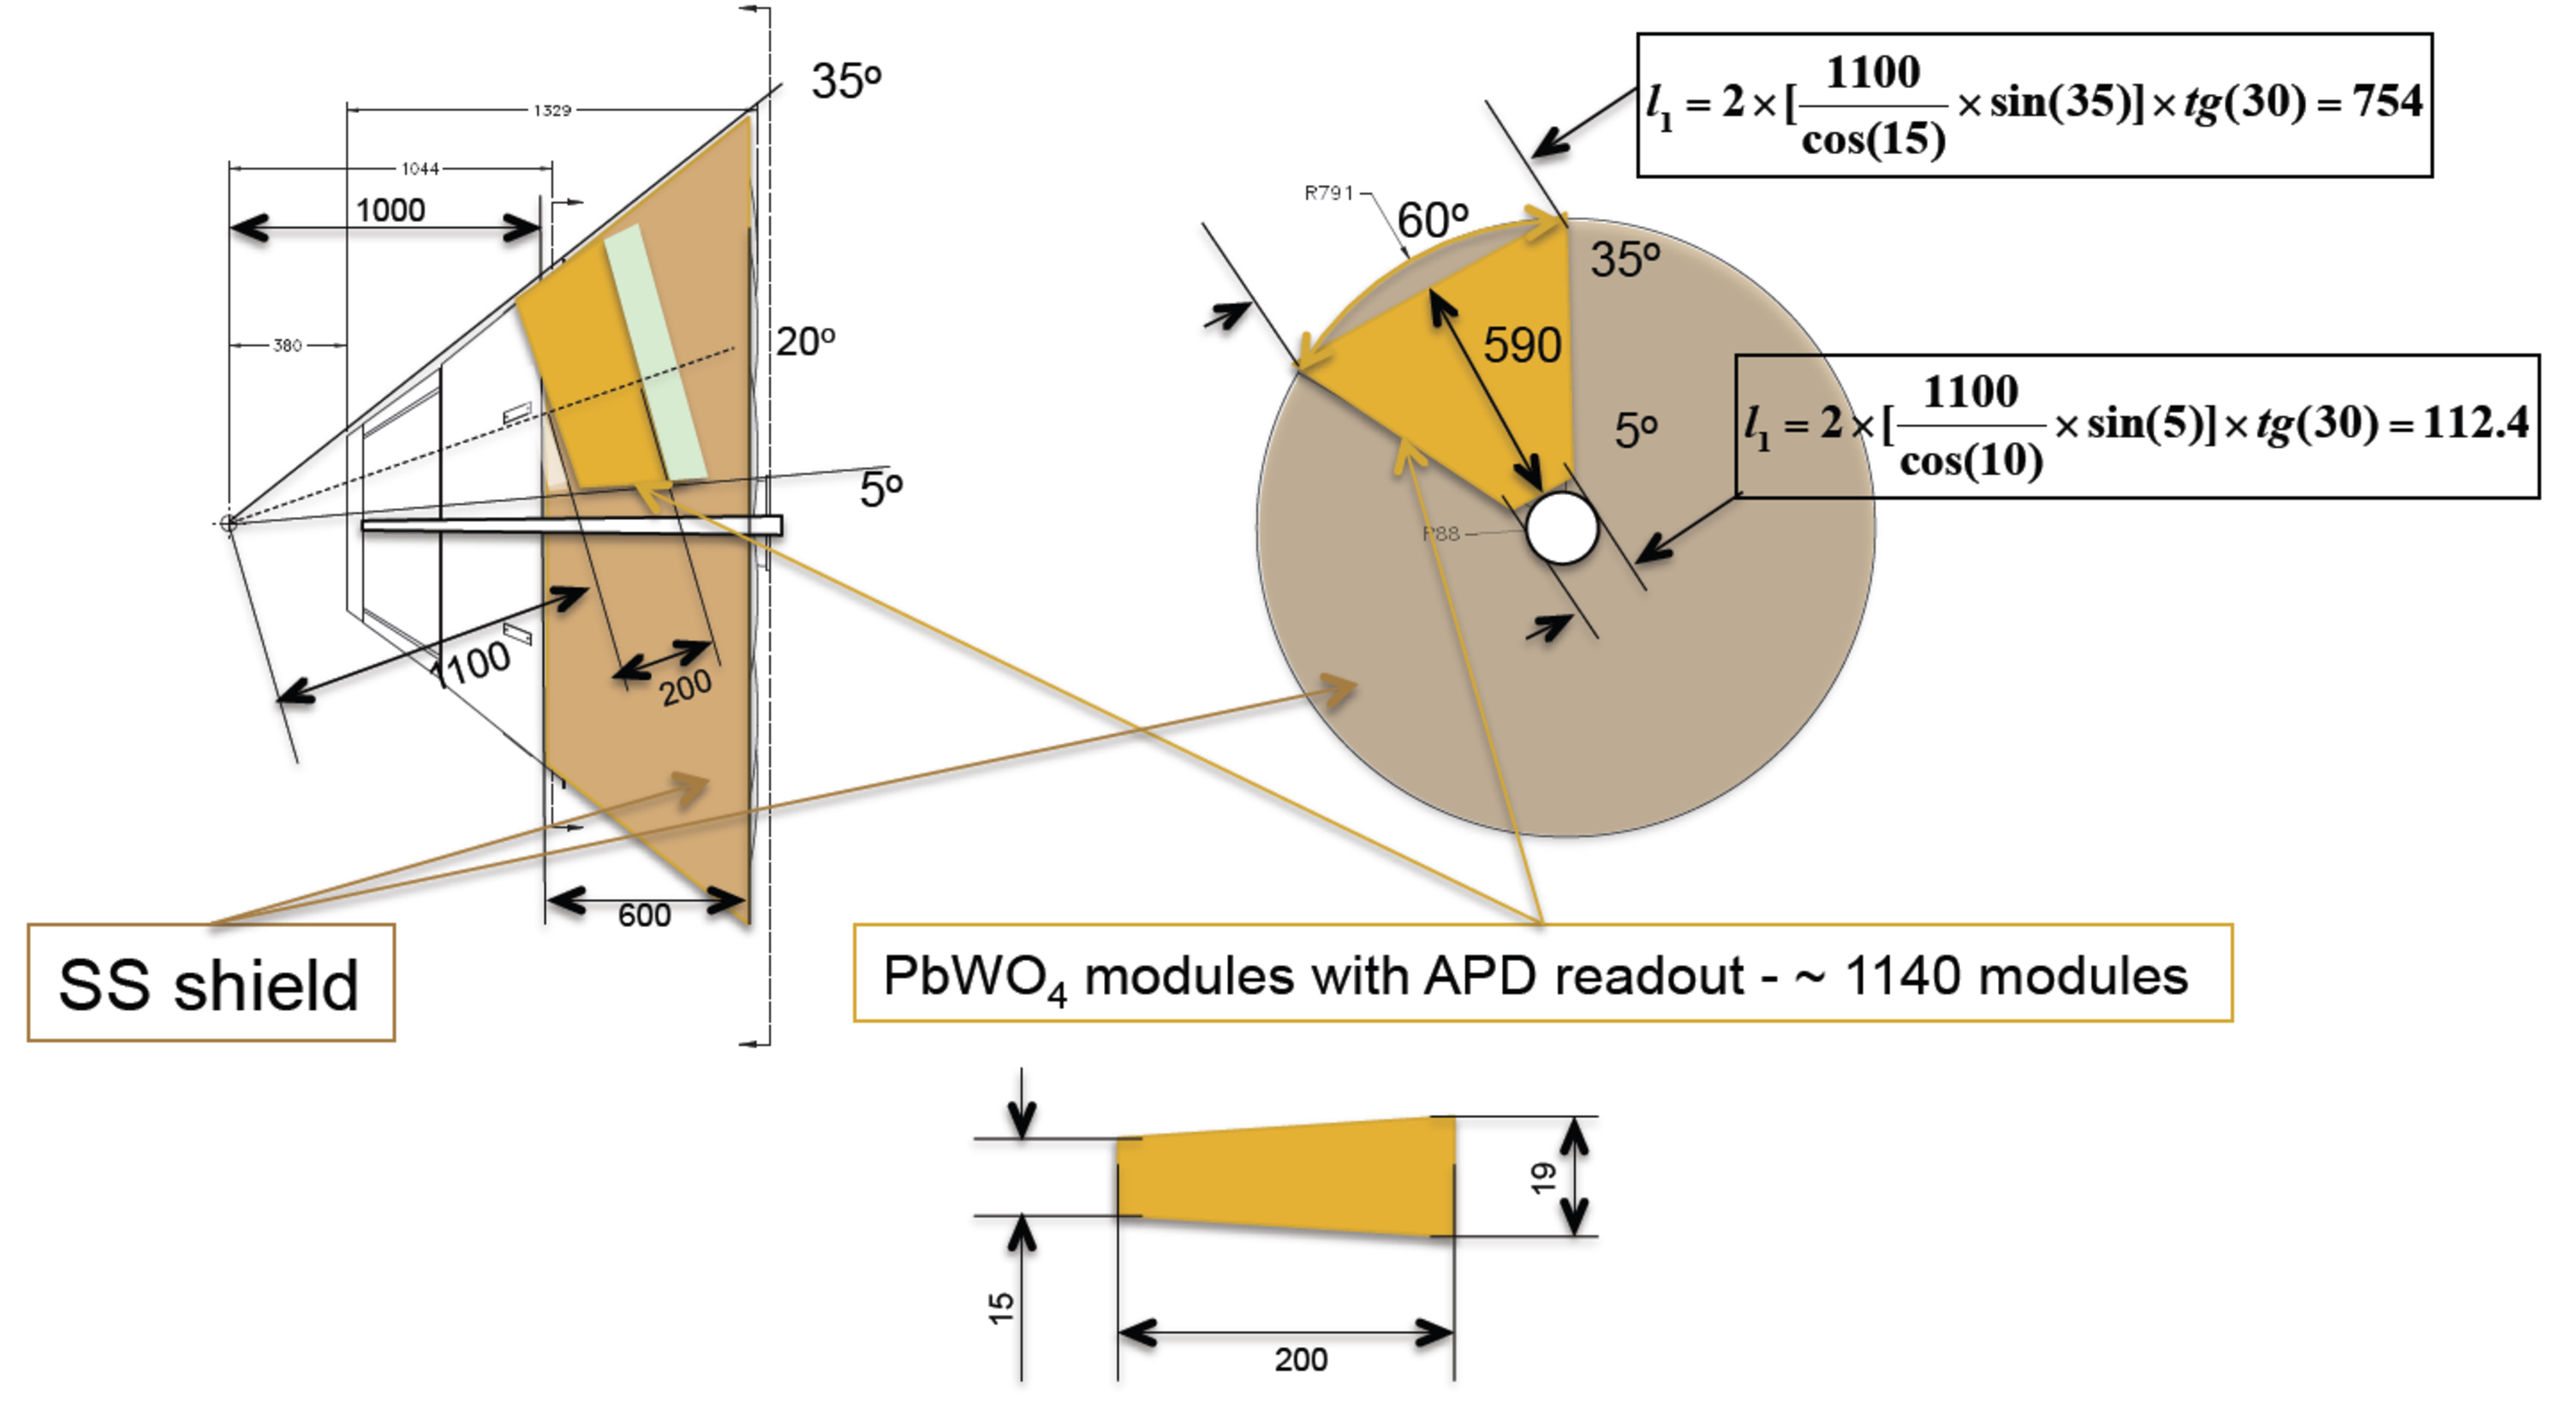
\includegraphics[width=1.\textwidth]{detector_concept.pdf}
\caption{The concept of the proposed shield and PbWO$_2$ calorimeter in the place of HTCC working gas. Dimensions on the figure are in mm, the size of PbWO$_4$ crystals are not optimized.}
\label{fig:shield}
\end{center}
\end{figure}


\clearpage

\subsection{Background Studies and Luminosity Limits}
L. Elouadrhiri, M. Ungaro


\section{Cross Sections, Acceptances, and Expected Rates}
\indent

For DDVCS and Bethe-Heitler cross section calculation the VGG code has been used \cite{vgg_code}. The same code was used in the event generator to simulate events for acceptance and resolution studies. The VGG code was modified to calculate Bethe-Heitler and DDVCS cross sections with di-muon final state. For J/$\psi$ electroproduction cross section estimate photoproduction cross section for 2-gluon exchange is used in conjunction with Vector Dominance Model (VDM). The detector acceptance was studied using a simple kinematic simulator \cite{fsgen} (see below for details). 

The acceptances and resolutions have been simulated using the modified version of the CLAS12 fast MC code \cite{fastmc}. A change was made to the CLAS12 FD simulation for angular resolution (for muons) due to the multiple scattering in the shielding/absorber. An additional $\sigma_C=0.01$ rad  multiple scattering term was added quadratically to the angular resolution calculation. The momentum of the tracks in FD will be measured with the forward drift chambers, then additional corrections will be applied to account for the energy loss in the absorber to calculate momentum at the production vertex (the energy loss in the absorber is not included in fast MC code).  

For electron detection a new detector was introduced in fast MC. The geometrical acceptance of the detector was confined within $\theta=5^\circ$ to $35^\circ$ and $\phi=0^\circ$ to $60^\circ$, where $\theta$ and $\phi$ are the polar and azimuthal angles of the particle, respectively. The energy resolution of $\sigma_E/E=3\%/\sqrt(E)$ and the angular resolution of $\sigma_{\theta(\phi)}=2$ mrad were taken from analysis of the performance of a similar calorimeter used for the Hall-B HPS experiment \cite{HPS}.


\subsection{DDVCS Cross Section and Expected Rates}
M. Guidal, M. Boer, R. Paremuzyan

To understand whether we will have good enough acceptance and reasonable rates, we performed Monte Carlo simulations 
of the $ep\rarr e^{\prime}\mu^{-}\mu^{+}p$ reaction. The incoming beam energy is assumed to be $11 \; GeV$.
%%%%%%%%%%%%%%%%%%%%%%%%%%%%%%%%%%%%%%% F I G U R E %%%%%%%%%%%%%%%%%%%%%%%%%%%%%%%%%%%%%%%%%%%%%%%%%
\begin{figure}[!htb]
 \centering
 \begin{subfigure}{0.48 \tw}
  \grinp[width=0.99\tw]{img/Qp2_Q2_gen_general2.pdf}
  \caption{}
  \label{fig:Qp2_Q2_gen_general2}
 \end{subfigure}
 \begin{subfigure}{0.48 \tw}
  \grinp[width=0.99\tw]{img/Qp2_Q2_rec_general2.pdf}
  \caption{}
  \label{fig:Qp2_Q2_rec_general2}
 \end{subfigure}
\begin{subfigure}{0.48 \tw}
  \grinp[width=0.99\tw]{img/Q2_xB_smear2.pdf}
  \caption{}
  \label{fig:Q2_xB_smear2}
 \end{subfigure}
 \begin{subfigure}{0.48 \tw}
  \grinp[width=0.99\tw]{img/tM_smear4.pdf}
  \caption{}
  \label{fig:tM_smear4}
 \end{subfigure}
 \caption{Top row: Generated (left) and reconstructed (right) distributions of "$Q^{\prime 2}$ vs $Q^{2}$".
 Bottom row: reconstructed "$Q^{2}$ vs $x_{B}$" (left) and $-t$ (right) when  $Q^{2} \in(2.5 - 3)\;GeV^{2}$ and $x_{B}\in(0.11 - 0.12)$.}
 \label{fig:kinematics_general}

\end{figure}
%%%%%%%%%%%%%%%%%%%%%%%%%%%%%%%%%%%%%%% F I G U R E %%%%%%%%%%%%%%%%%%%%%%%%%%%%%%%%%%%%%%%%%%%%%%%%%
Simulations were limited in the $Q^{2}\in(0.8-7.2)\;GeV^{2}$ and $Q^{\prime 2}\in(1.8-4.8)\;GeV^{2}$ region.
Generated DDVCS events were passed through the CLAS12 FastMC Acceptance package (described in a previous section).
In Fig.\ref{fig:kinematics_general} shown distributions of some kinematic variables: Generated (top left) and reconstructed (top right) 
"$Q^{\prime 2}$ vs $Q^{2}$" distributions, "$Q^{2}$ vs $x_{B}$" is the bottom left, and the bottom right represent $-t$ distribution 
when $Q^{2}$ and $x_{B}$ are in the following region $Q^{2} \in(2. - 3)\;GeV^{2}$ and $x_{B}\in(0.11 - 0.2)$.

In this LOI we will present estimated rates and statistical uncertainties of beam spin asymmetries as a function of
$\Phi_{L}$ by fixing kinematic bin $Q^{2} \in(2. - 3.)\;GeV^{2}$, $-t\in (0.1 - 0.4)\; GeV^{2}$, $x_{B}\in(0.11 - 0.2)$ (See 
bottom row of Fig.\ref{fig:kinematics_general}), and 
varying $Q^{\prime 2}$ ($Q^{\prime 2} = {2.,\; 2.8,\;  3.6} \;GeV^{2}$). Limits are also shown in 

%%%%%%%%%%%%%%%%%%%%%%%%%%%%%%%%%% MC generator description %%%%%%%%%%%%%%%%%%%%%%%%%%%%%%%%%%%%%%%%
Each generated event contains 7 fold cross section, which is used for estimation of rates.
\begin{equation}
\frac{\dstl d\sigma}{\dstl dQ^{2} dt dQ^{\prime 2} dx_{B} d\Phi_{L} d\Phi_{cm} d\Theta_{cm}} 
\end{equation}
Where angles $\Phi_{L}$, $\Phi_{CM}$ and $\Theta_{CM}$ are shown on Fig. \ref{fig:DDVCS_Angles}, and their definition is described in the caption
of the figure.
%%%%%%%%%%%%%%%%%%%%%%%%%%%%%%%%%%%%%%% F I G U R E %%%%%%%%%%%%%%%%%%%%%%%%%%%%%%%%%%%%%%%%%%%%%%%%%
\begin{figure}[!htb]
 \centering
 \begin{subfigure}{0.48 \tw}
  \grinp[width=0.99\tw]{Angles_DDVCS1.pdf}
  \caption{}
  \label{fig:DDVCS_Angles1}
 \end{subfigure}
 \begin{subfigure}{0.48 \tw}
  \grinp[width=0.99\tw]{Angles_DDVCS2.pdf}
  \caption{}
  \label{fig:DDVCS_Angles2}
 \end{subfigure}
\caption{Representation of DDVCS angles. $\Phi_{L}$ is the angle between beam scattering and hadronic planes (left figure), $\Phi_{CM}$ 
is the angle between decay lepton and hadronic planes (left figure) and $\Theta_{CM}$ (right figure) is the angle of the negative
decay lepton w.r.t. scattered proton momentum, in the frame where timelike photon is at rest.}
\label{fig:DDVCS_Angles}
\end{figure}
%%%%%%%%%%%%%%%%%%%%%%%%%%%%%%%%%%%%%%% F I G U R E %%%%%%%%%%%%%%%%%%%%%%%%%%%%%%%%%%%%%%%%%%%%%%%%%

The cross section represent the sum of three cross sections DDVCS, BH and their interference term.
%Calculation of cross section is not fast and it is very unpractical to calculate cross section for each generated event,
%instead the cross section is calculated in a discrete values of $Q^{2}$, $Q^{\prime 2}$, $t$, $\Phi_{L}$, $\Phi_{CM}$ and $\Theta_{CM}$, then
%cross section is extrapolated using the two (in each variable) closest values of already defined cross section.
Kinematic distribution of final state particles, when all of them ($e^{-},\;\mu^{-}$ and $\mu^{+}$) are detected, are shown in 
Fig.\ref{fig:particle_kinematic_distr}, where
\begin{figure}[!htb]
 \centering
  \begin{subfigure}{0.48 \tw}
  \grinp[width=0.99\tw]{img/th_P_mum_rec4.pdf}
  \caption{}
  \label{fig:th_P_mum_rec4}
 \end{subfigure}
 \begin{subfigure}{0.48 \tw}
  \grinp[width=0.99\tw]{img/th_P_mup_rec4.pdf}
  \caption{}
  \label{fig:th_P_mup_rec4}
 \end{subfigure}
 \begin{subfigure}{0.48 \tw}
  \grinp[width=0.99\tw]{img/th_P_em_rec2.pdf}
  \caption{}
  \label{fig:th_P_em_rec2}
 \end{subfigure}
 \begin{subfigure}{0.48 \tw}
  \grinp[width=0.99\tw]{img/MM_smear1.pdf}
  \caption{}
  \label{fig:MM_smear1}
 \end{subfigure}
 \caption{ $\theta$ vs $P$ distributions for detected $\mu^{-}$ (a), $\mu^{+}$ (b) and $e-$ (c).
(d) is the missing mass of detected $e^{-}\mu^{-}\mu^{+}$ system.}
\label{fig:particle_kinematic_distr}
\end{figure}
a, b, and c represent "$\theta$ vs $P$" distributions for $\mu^{-}$, $\mu^{+}$ and $e^{-}$ respectively, and d is the
missing mass of detected $e^{-}\mu^{-}\mu^{+}$ system.
As one can see because of different kinematics of $J/\Psi$ (narrow and high $M(\mu^{-}\mu^{+})$ mass region) and DDVCS (wide and lower $M(\mu^{-}\mu^{+})$),
kinematic distributions "$\theta$ vs $P$" are not quite similar,
however missing mass resolution is still as good as in $J/\Psi$
case (see Figs. \ref{fig:jp_mukine} and \ref{fig:jp_mres}), and will allow ensure exclusivity of the reaction.

For the aforementioned kinematic bin, the acceptance and expected rates in three bins of $Q^{\prime 2}$ are shown in Fig.\ref{fig:Acc_and_rates_Qp2}
As one can see the acceptance is not bad and it is around $2.5\%$.
\begin{figure}[!htb]
 \centering
   \begin{subfigure}{0.48 \tw}
  \grinp[width=0.99\tw]{img/Acc_Qp2.pdf}
  \caption{}
  \label{fig:Acc_Qp2}
 \end{subfigure}
 \begin{subfigure}{0.48 \tw}
  \grinp[width=0.99\tw]{img/h_Qp2_rates1.pdf}
  \caption{}
  \label{fig:h_Qp2_rates1}
 \end{subfigure}
\caption{Acceptance and expected rates for different bins of $Q^{\prime 2}$ (left)}
\label{fig:Acc_and_rates_Qp2}
\end{figure}
Later to estimate statistical uncertainties on the Beam Spin asymmetries, each $Q^{\prime 2}$ bin is divided into 12 bins on $\Phi_{L}$, and for each bin 
counts and statistical error-bars on asymmetry as a function of $\Phi$
 are shown in \ref{fig:counts_and_errorbars0}, \ref{fig:counts_and_errorbar1} and \ref{fig:counts_and_errorbars2}.
 These estimations were performed assuming $10^{37}cm^{-2}s^{-}$ luminosity and 100 days of running.
%%%%%%%%%%%%%%%%%%%%%%%%%%%%%%%%%%%%%%% F I G U R E %%%%%%%%%%%%%%%%%%%%%%%%%%%%%%%%%%%%%%%%%%%%%%%%%
\begin{figure}[!htb]
 \centering
   \begin{subfigure}{0.48 \tw}
  \grinp[width=0.99\tw]{img/PHI_DVCS_rates_0.pdf}
  \caption{}
  \label{fig:PHI_DVCS_rates_0}
 \end{subfigure}
 \begin{subfigure}{0.48 \tw}
  \grinp[width=0.99\tw]{img/Asym_errorbars_0.pdf}
  \caption{}
  \label{fig:Asym_errorbars_0}
 \end{subfigure}\\
\caption{Count rates (left) and statistic error-bars for (right) for the $Q^{\prime2}(1.8-2.4); GeV^{2}$ bin}
\label{fig:counts_and_errorbars0}
\end{figure}
%%%%%%%%%%%%%%%%%%%%%%%%%%%%%%%%%%%%%%% F I G U R E %%%%%%%%%%%%%%%%%%%%%%%%%%%%%%%%%%%%%%%%%%%%%%%%%
\begin{figure}[!htb]
 \centering
   \begin{subfigure}{0.48 \tw}
  \grinp[width=0.99\tw]{img/PHI_DVCS_rates_1.pdf}
  \caption{}
  \label{fig:PHI_DVCS_rates_1}
 \end{subfigure}
 \begin{subfigure}{0.48 \tw}
  \grinp[width=0.99\tw]{img/Asym_errorbars_1.pdf}
  \caption{}
  \label{fig:Asym_errorbars_1}
 \end{subfigure}\\
\caption{Count rates (left) and statistic error-bars (right) for the $Q^{\prime2}(2.4 - 3.2); GeV^{2}$ bin}
\label{fig:counts_and_errorbar1}
\end{figure}
%%%%%%%%%%%%%%%%%%%%%%%%%%%%%%%%%%%%%%% F I G U R E %%%%%%%%%%%%%%%%%%%%%%%%%%%%%%%%%%%%%%%%%%%%%%%%%
\begin{figure}[!htb]
 \centering
   \begin{subfigure}{0.48 \tw}
  \grinp[width=0.99\tw]{img/PHI_DVCS_rates_2.pdf}
  \caption{}
  \label{fig:PHI_DVCS_rates_2}
 \end{subfigure}
 \begin{subfigure}{0.48 \tw}
  \grinp[width=0.99\tw]{img/Asym_errorbars_2.pdf}
  \caption{}
  \label{fig:Asym_errorbars_2}
 \end{subfigure}\\
\caption{Count rates (left) and statistic error-bars (right) for the $Q^{\prime2}(3.2 - 4); GeV^{2}$ bin}6
\label{fig:counts_and_errorbars2}
\end{figure}
%%%%%%%%%%%%%%%%%%%%%%%%%%%%%%%%%%%%%%% F I G U R E %%%%%%%%%%%%%%%%%%%%%%%%%%%%%%%%%%%%%%%%%%%%%%%%%
% \begin{figure}[!htb]
%  \centering
%    \begin{subfigure}{0.48 \tw}
%   \grinp[width=0.99\tw]{img/PHI_DVCS_rates_3.pdf}
%   \caption{}
%   \label{fig:PHI_DVCS_rates_3}
%  \end{subfigure}
%  \begin{subfigure}{0.48 \tw}
%   \grinp[width=0.99\tw]{img/Asym_errorbars_3.pdf}
%   \caption{}
%   \label{fig:Asym_errorbars_3}
%  \end{subfigure}\\
% \caption{Count rates (left) and statistic error-bars (right) for the $Q^{\prime2}(4. - 4.8); GeV^{2}$ bin}
% \label{fig:counts_and_errorbars3}
% \end{figure}
%%%%%%%%%%%%%%%%%%%%%%%%%%%%%%%%%%%%%%% F I G U R E %%%%%%%%%%%%%%%%%%%%%%%%%%%%%%%%%%%%%%%%%%%%%%%%%

\subsection{J/$\Psi$ Electroproduction}
N. Baltzel, F-X. Girod, S. Stepanyan
\indent

The main goal  for J/$\Psi$ electroproductionis to study t-dependence of the cross section for different Q$^2$ ranges. In order to calculate acceptances, cross sections, and the rates, coverage in kinematics is studied for events when electron, $\mu^+$ and $\mu^-$ are detected, and electron has momentum $p>0.5$ GeV/c. In Fig.\ref{fig:jp_e0p5_q2w} Q$^2$ vs W (total invariant mass) is shown. Because of rather limited energy range, we will integrate the full W-rage for a given Q$^2$ bin. So the future selection proceeds for W-range $4.025 < W < 4.525$ GeV.   

\begin{figure}[htbp]
\begin{center} 
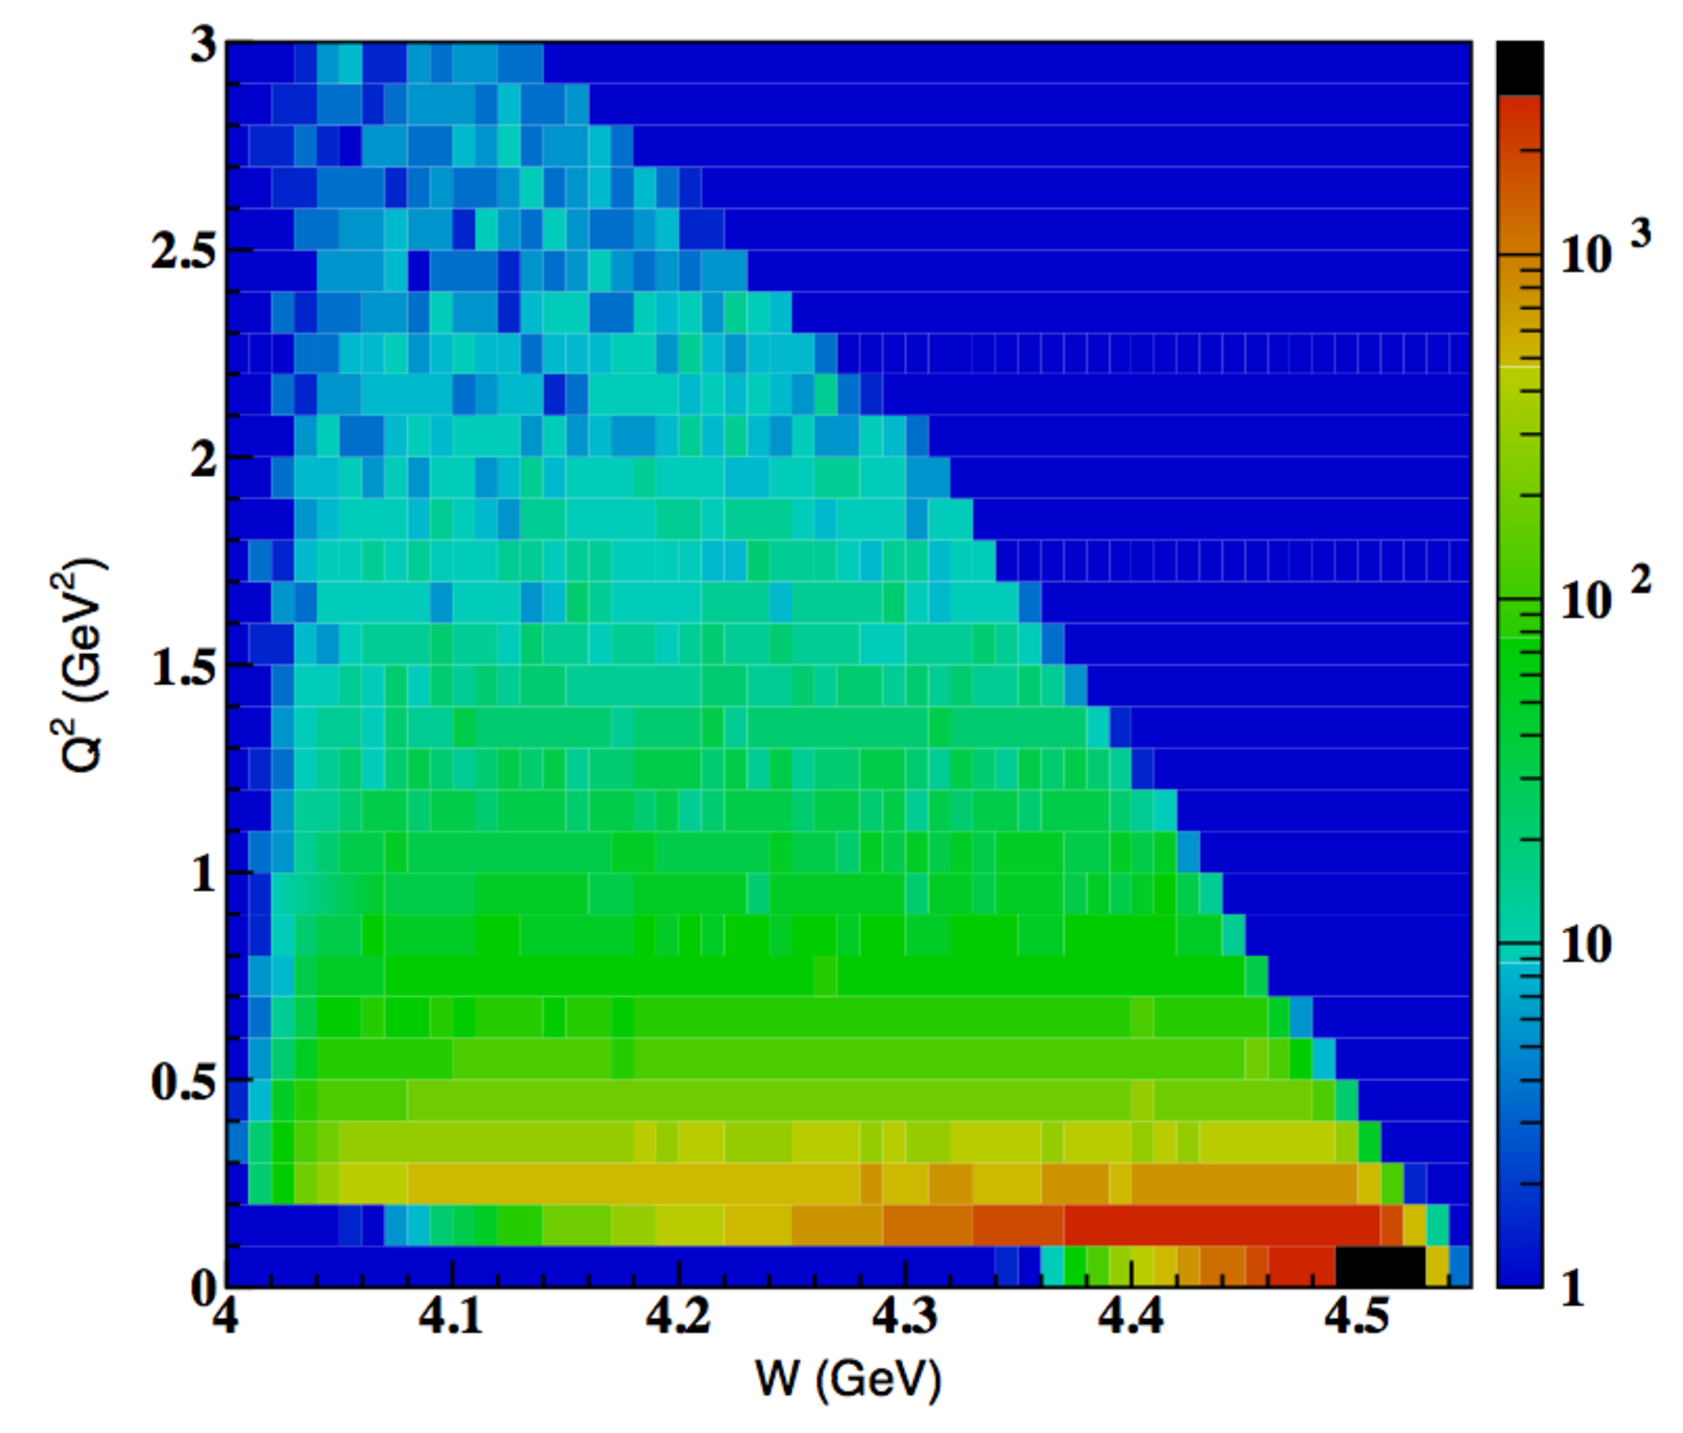
\includegraphics[width=0.8\textwidth]{jpsi_q2_w_emin_0p5.pdf}
\caption{Q$^2$ vs. W  dependance for events with electron, and both muons detected. There is $0.5$ GeV/c minimum momentum cut for the electrons.}
\label{fig:jp_e0p5_q2w}
\end{center}
\end{figure}

\begin{figure}[htbp]
\begin{center} 
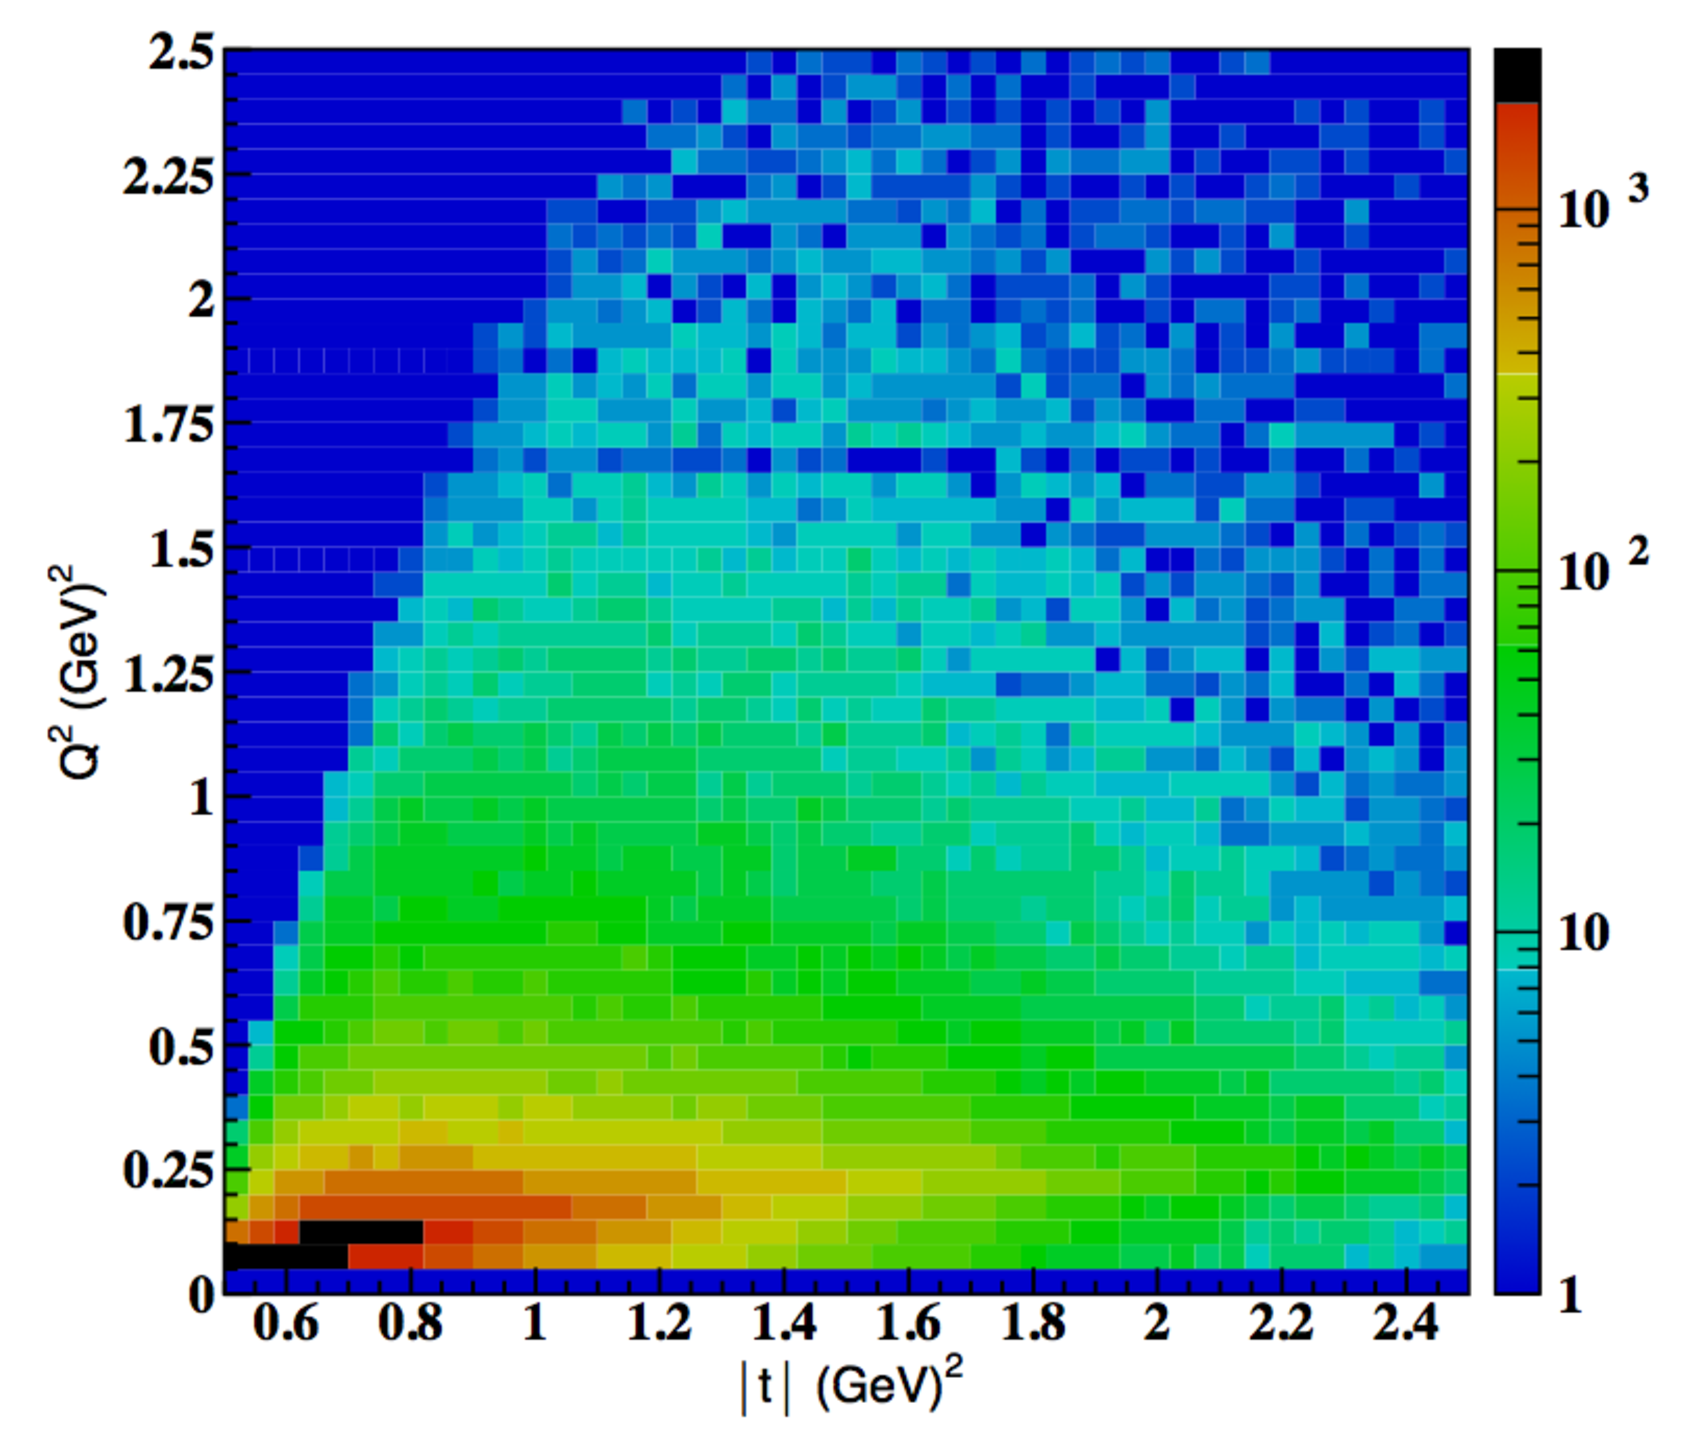
\includegraphics[width=0.8\textwidth]{jpsi_q2_t_w4025_w4525.pdf}
\caption{Q$^2$ vs. t  dependance for $4.025 < W < 4.525$ GeV.}
\label{fig:jp_q2t}
\end{center}
\end{figure}

Fig.\ref{fig:jp_q2t} shows Q$^2$ - t landscape in the selected W-range. Based on this distribution the t-dependance was studied for three bins of Q$^2$, $0.1<$Q$^2 <0.3$ GeV$^2$, $0.3<$Q$^2 <1.$ GeV$^2$, and $1<$Q$^2 < 2.5$ GeV$^2$. The average values of Q$^2$ in each bin are $0.19$ GeV$^2$,  $0.5$ GeV$^2$, and $1.45$ GeV$^2$, respectively. For these studies cross sections are calculated using bin average values for W, Q$^2$, and $t$.


\subsubsection{Cross Section Formalism.}
\indent

The cross section of $t$-channel meson electroproduction on the
nucleon (see diagram on Figure \ref{fig:diagn}), integrated over the
azimuthal angle between electron and hadron planes, can be presented 
as a sum of cross sections for transversely ($\sigma_T$), and
longitudinally ($\sigma_L$) polarized photons: 
\begin{eqnarray}
\label{eq:cse}
{d\sigma _{eN \rightarrow eM^0 N}  \over dQ^2dWdt}=
\Gamma_W\cdot ({d\sigma_T \over dt}~+~\epsilon{d\sigma_L \over dt}) \ .
\end{eqnarray}
Here $\Gamma_W$ is the flux of virtual photons and is defined as:
\begin{eqnarray}
\label{eq:flux}
\Gamma_W=
{\alpha\over 4\pi}\cdot{W^2-m^2\over m^2E^2}\cdot{W\over Q^2}\cdot 
{1\over 1-\epsilon}  \ .
\end{eqnarray}
In the equations above, $\epsilon$ is the virtual photon polarization and is
given by:
\begin{eqnarray}
\label{eq:eps}
\epsilon = \left( 1+2{Q^2+q^{02}\over 4EE'-Q^2} \right)^{-1} \ .
\end{eqnarray}
%%%%%%%%%%%%%%%%%%% Figure : Fdia %%%%%%%%%%%%%%%%%%%%%%%
\begin{figure}[htbp]
\begin{center} 
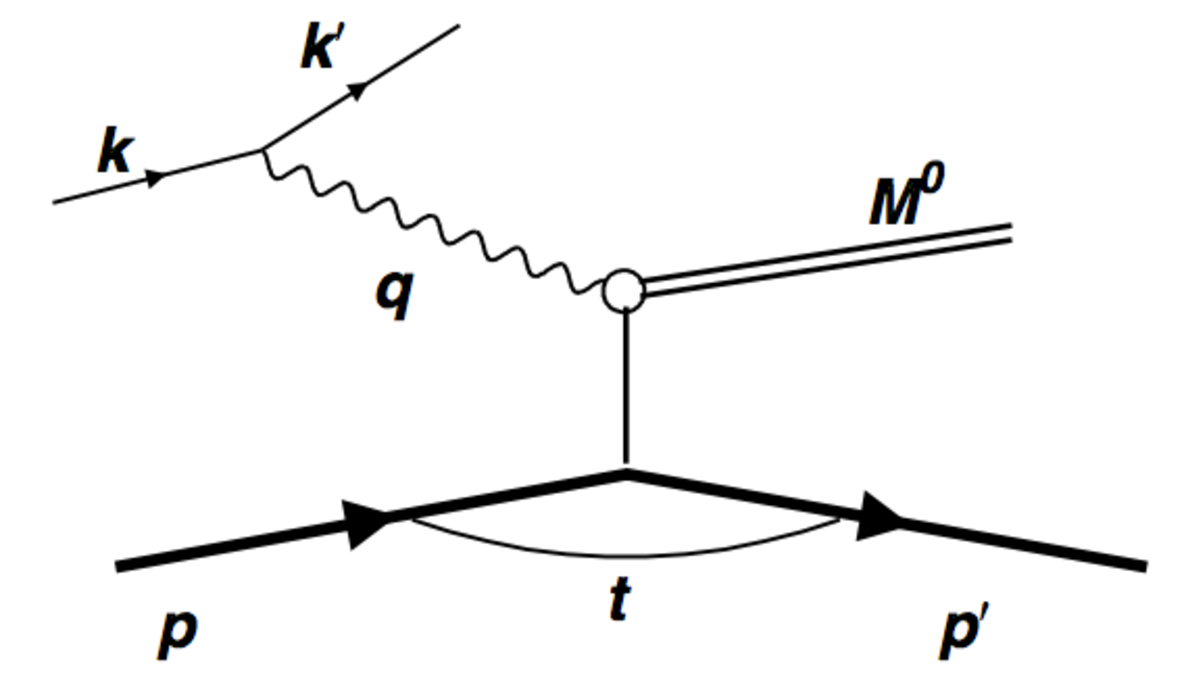
\includegraphics[width=0.7\textwidth]{ep_pm0.pdf}
\caption{Diagram for electroproduction of a $t$-channel meson on the nucleon.}
\label{fig:diagn}
\end{center}
\end{figure}
%%%%%%%%%%%%%%%%%%%%%%%%%%%%%%%%%%%%%%%%%%%%%%%%%%%%

The other kinematical variables are: electron transfered momentum squared
$Q^2=-q^{\mu 2}$ were $q^\mu=(k^\mu-k^{\prime \mu})$ is the four-momentum 
of the virtual photon, and $k^\mu$($k^{\prime\mu}$) is the 
four-momentum of incoming (outgoing) electron. In Eq.(\ref{eq:cse}) $t$
is the transferred momentum squared to the target, and the mass squared 
of the virtual photon hadron system, $W^2$, is:
\begin{eqnarray}
\label{eq:w}
W^2~=~m^2+2mq^0 - Q^2 \ ,
\end{eqnarray}
$m$ is the nucleon mass.

Using vector meson dominance (VDM) one can relate $\sigma_T$
and $\sigma_L$ to the photoproduction cross section \cite{vdm}.
The relation for $\sigma_T$ is:
\begin{eqnarray}
\label{eq:st}
\sigma_T ~=~  \left( {m_{J/\Psi}^2\over 
m_{J/\Psi}^2+Q^2} \right) ^2\cdot \sigma_{\gamma N \rightarrow M^0N} \ ,
\end{eqnarray}
and for $\sigma_L$:
\begin{eqnarray}
\label{eq:sl}
\sigma_L~=~\left( {m_{J/\Psi}^2\over m_{J/\Psi}^2+Q^2} 
\right) ^2\cdot 
{Q^2\over m_{J/\Psi}^2}\cdot (1-x)^2
\cdot \xi(Q^2,\nu)\cdot \sigma_{\gamma N \rightarrow M^0p} \ ,
\end{eqnarray}
where $m_{J/\Psi}$ is the $J/\Psi$ meson mass. 
$\xi(Q^2,\nu)$ scales the model to the data, and is taken to be $0.5$ for our calculations.  
The $x=Q^2/(2qp)$ where $p$ is the four-momentum of the target nucleon. 
The $\sigma_{\gamma N
\rightarrow M^0N^\prime}$ is the photoproduction cross section. For our calculations we used 2-gluon formalism for the differential cross section from \cite{brodsky:2000zc}:

\begin{eqnarray}
{d\sigma\over {dt}} = N_{2g}\nu{(1-x)^2\over{R^2M^2}}F^2_{2g}(t)(s-m_p^2)^2
\end{eqnarray}
where where $F_{2g}(t)$ is the proton form factors that take into account the fact that the three target quarks recombine into the final proton after the emission of two gluons. The $N_{2g}$ is scaling factor to saturate measured cross sections, $M$ is the mass of the $c\bar c$, $R$ is the proton radius (taken as $1$ fm, $s$ is the center mass energy square and the $x$ is the fraction of the proton momentum carried by the valence quark.  

\begin{figure}[htbp]
\begin{center}
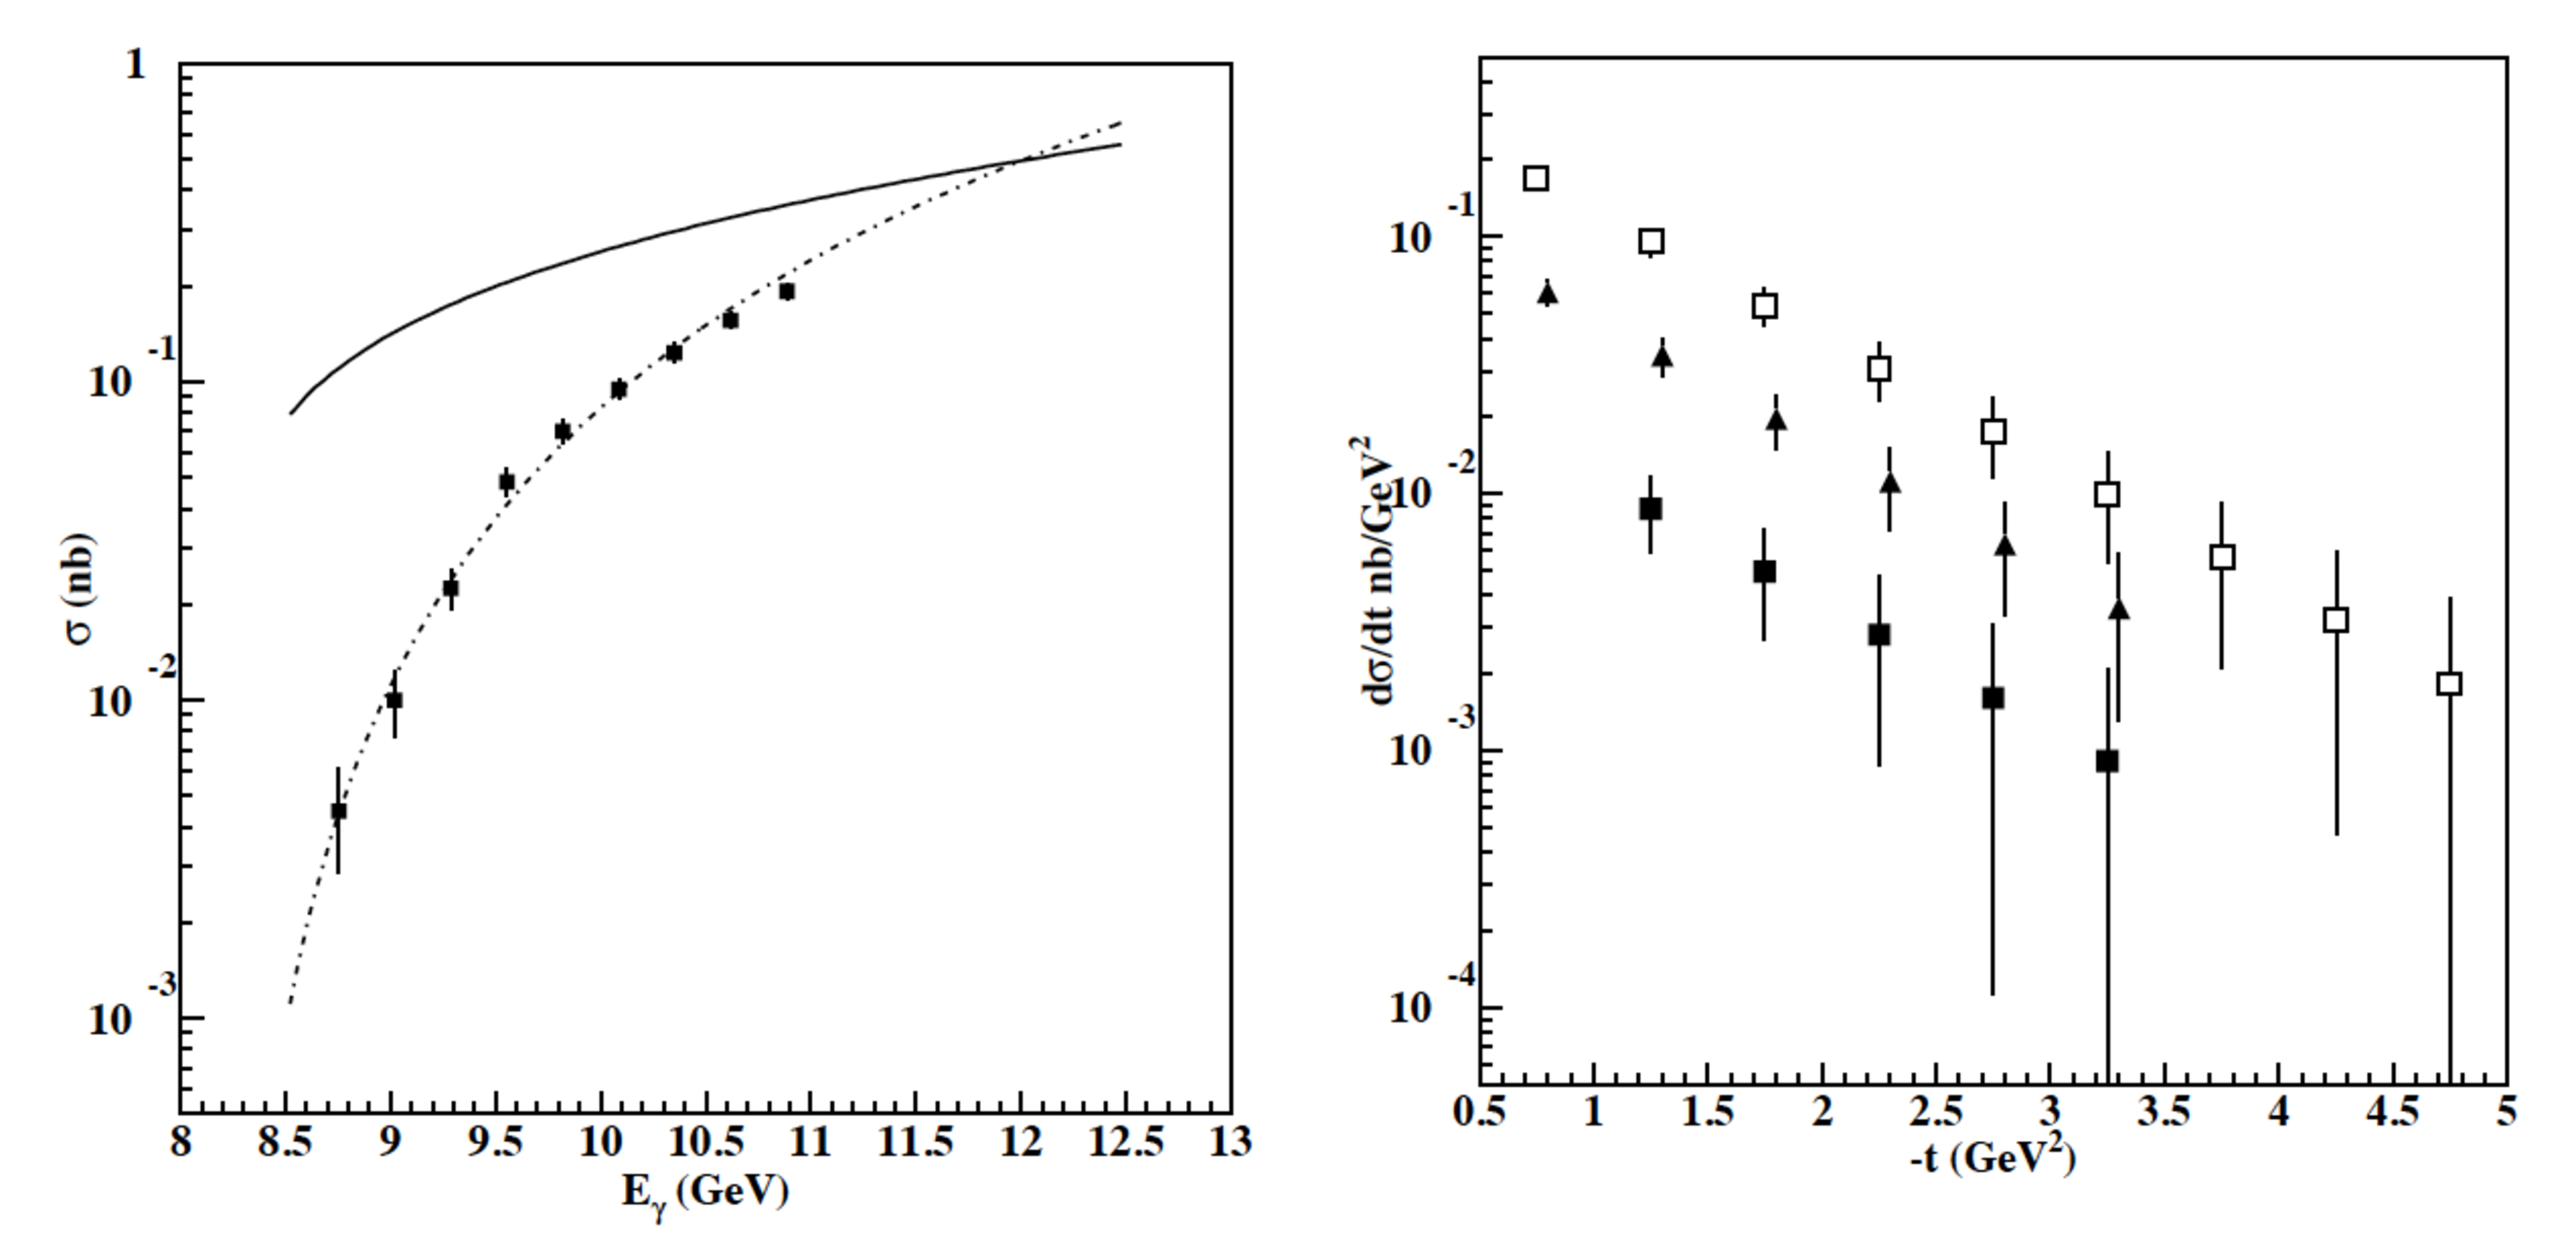
\includegraphics[width=1\textwidth]{jpsi_photo.pdf}
\end{center}
\caption{The cross section of exclusive $J/\psi$ photoproduction in 100 days of running from \cite{tcs_clas12}. On the left: total cross section as a function of the incoming photon energy. The curves are calculated according to cross section formulas in Ref. \cite{brodsky:2000zc}. On the right: Differential cross section as a function of the four-momentum transfer $-t$ for three bins of $s$. The dashed line and the filled squares are for $s=17.55$ to $18.05$ GeV$^2$, the dotted line and the inverted filled triangles are for $s=19.05$ to $19.55$ GeV$^2$, and the dashed-dotted line and the open squares are for $s=21.05$ to $21.55$ GeV$^2$.}
\label{fig:jpsixs2}
\end{figure}


This cross section model has been used to calculate cross sections for the experiment E-12-12-001 \cite{e1212001}. The $t$-distribution for exclusive $J/\Psi$ photoproduction from E12-12-001 proposal is shown in Fig.~\ref{fig:jpsixs2}. The same code was used to calculate cross sections for the electroproduction cross section in the kinematics of the present proposal.


\label{acc_simulations}
\indent


\clearpage

\subsubsection{Acceptance simulations for J/$\Psi$}
\indent

The generator used for J/$\Psi$ acceptance studies simulates multi-particle final states in photo- and electro production reactions. It has correct decay channels and branching ratios for most of particles listed in PDG (Lund/Jetset \cite{lepto}) and allows to set the kinematic dependencies, e.g. Q$^2$ and $t$. The reaction: 
\begin{eqnarray}
ep\to e^\prime~J/\Psi~p^\prime\to e^\prime\mu^+\mu^-p^\prime
\end{eqnarray}
was simulated with the following conditions:
\begin{itemize}
\item beam energy $E=11$ GeV
\item electron four momentum transferred dependence $1/{Q^4}$ ($Q^2=-q^2=-(k_i-k_f)^2$, where $k_{i(f)}$ is the initial (final) four momentum of the electron)
\item exponential dependence for the squared four-momentum transfer from initial to final state proton, $e^{3t}$, ($t=(p_i-p_f)^2$, where $p_i$ and $p_f$ are four momenta of the initial and final state protons)
\end{itemize}

The Q$^2$- and t-dependences as they have been generated initially and their form after the electron is selected in the calorimeter detection range are shown in Fig.\ref{fig:jp_sim}. The cutoff on maximum Q$^2$ and t after electron selection are due to the minimum momentum, $p_{min}=0.5$ GeV, and the maximum angel, $\theta_{max}=35^\circ$ limits.

\begin{figure}[htbp]
\begin{center}
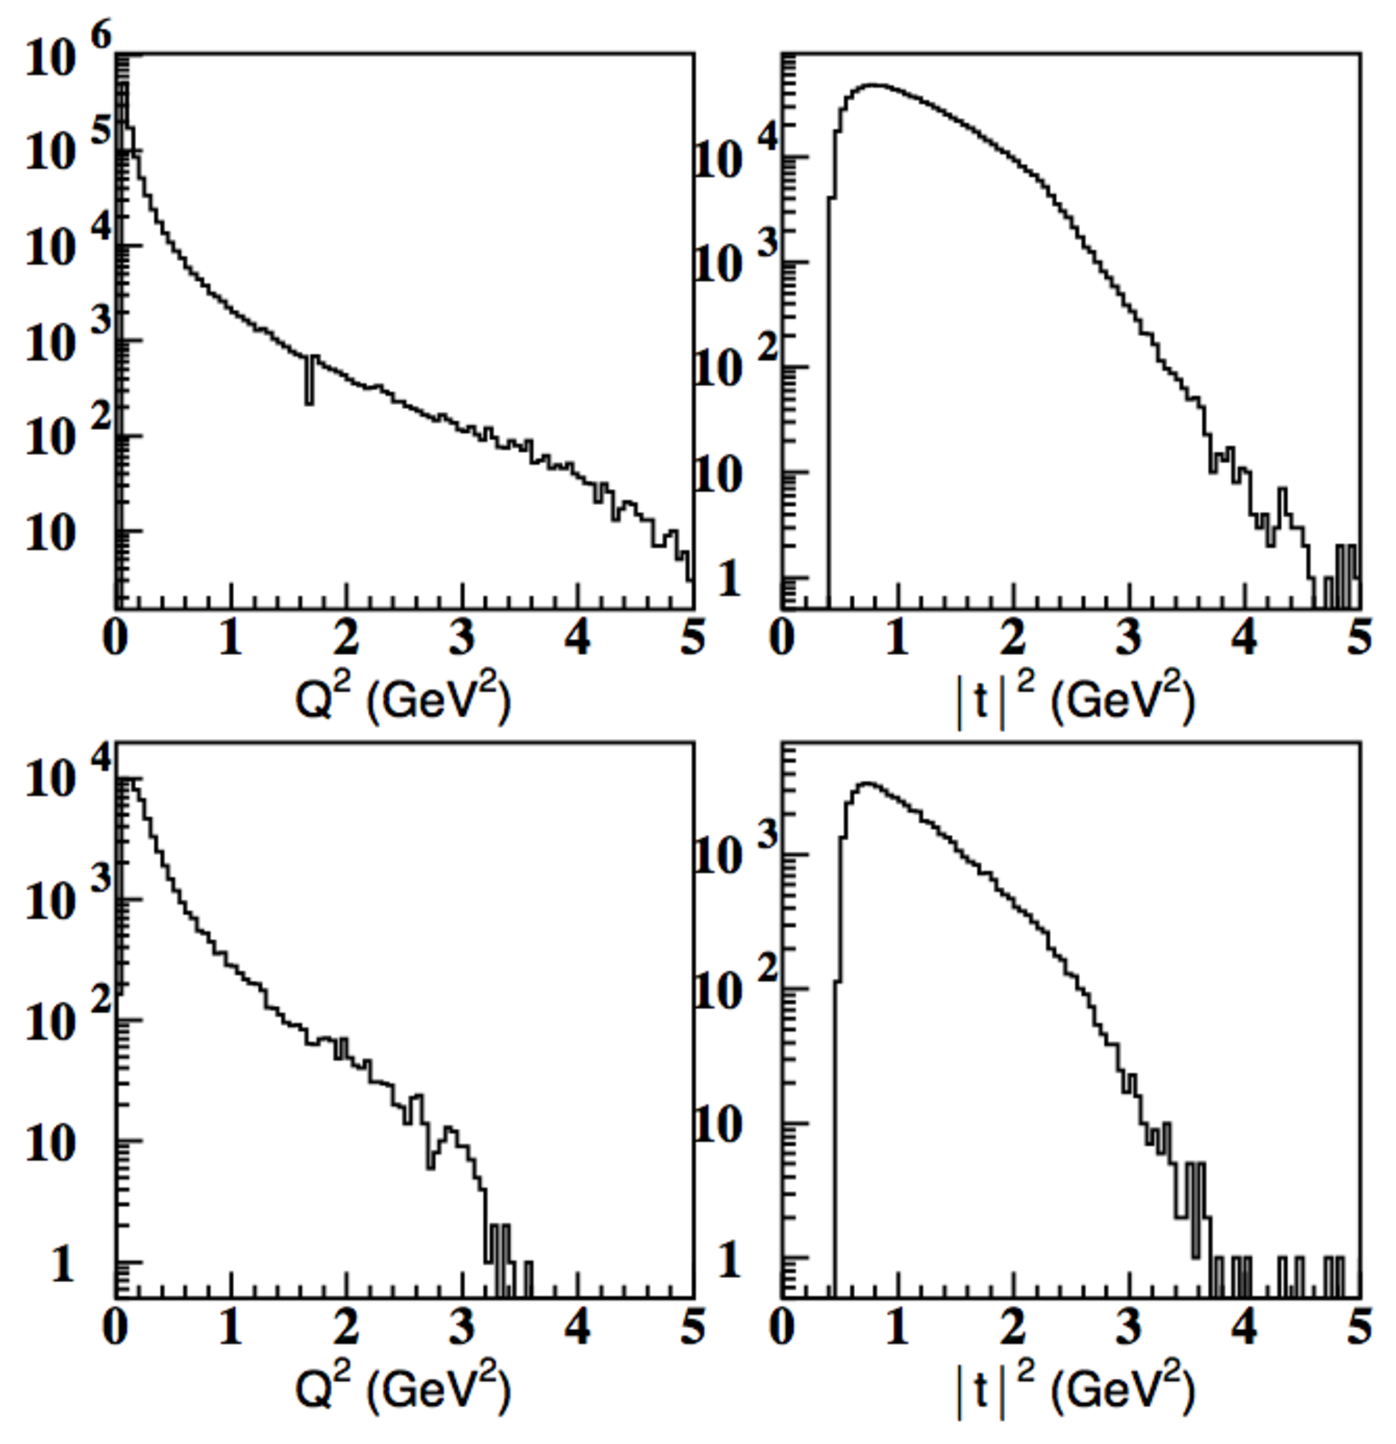
\includegraphics[width=0.8\textwidth]{jpsi_q2_t_sim.pdf}
\caption{Simulated Q$^2$ and $t$ distributions, top. On the bottom panels the same distributions when electron is detected in the calorimeter.  }
\label{fig:jp_sim}
\end{center}
\end{figure}

In Fig.\ref{fig:jp_kine}, momentum vs. scattering angle distributions for final state particles in the reaction $ep\to e^\prime p^\prime J/\Psi$ are shown. Due to large momentum transfer, near threshold  production, recoil protons will scatter at forward direction and will not be detected. Electrons will be detected in the calorimeter as was described above in the angular rage $5^\circ < \theta_e <35^\circ$ with momentum $p>0.5$ GeV/c. The muons are produced mostly in forward angles ($\theta_\mu<40^\circ$), bottom left panel of Fig.\ref{fig:jp_kine}, and remain in the same momentum-angular space with electrons in the calorimeter, bottom right panel. The CLAS12 FD that can detect changed tracks in angular range $5^\circ < \theta <35^\circ$ is well suited for detecting muons from presented reaction. In Fig.\ref{fig:jp_mukine} momentum vs scattering angle of $\mu^+$ and $\mu^-$ are shown. Due to large momentum there is not much difference in detection acceptance for negatively and positively charged tracks at forward angles due to the magnetic field and the CLAS12 detector acceptances.

\begin{figure}[htbp]
\begin{center}
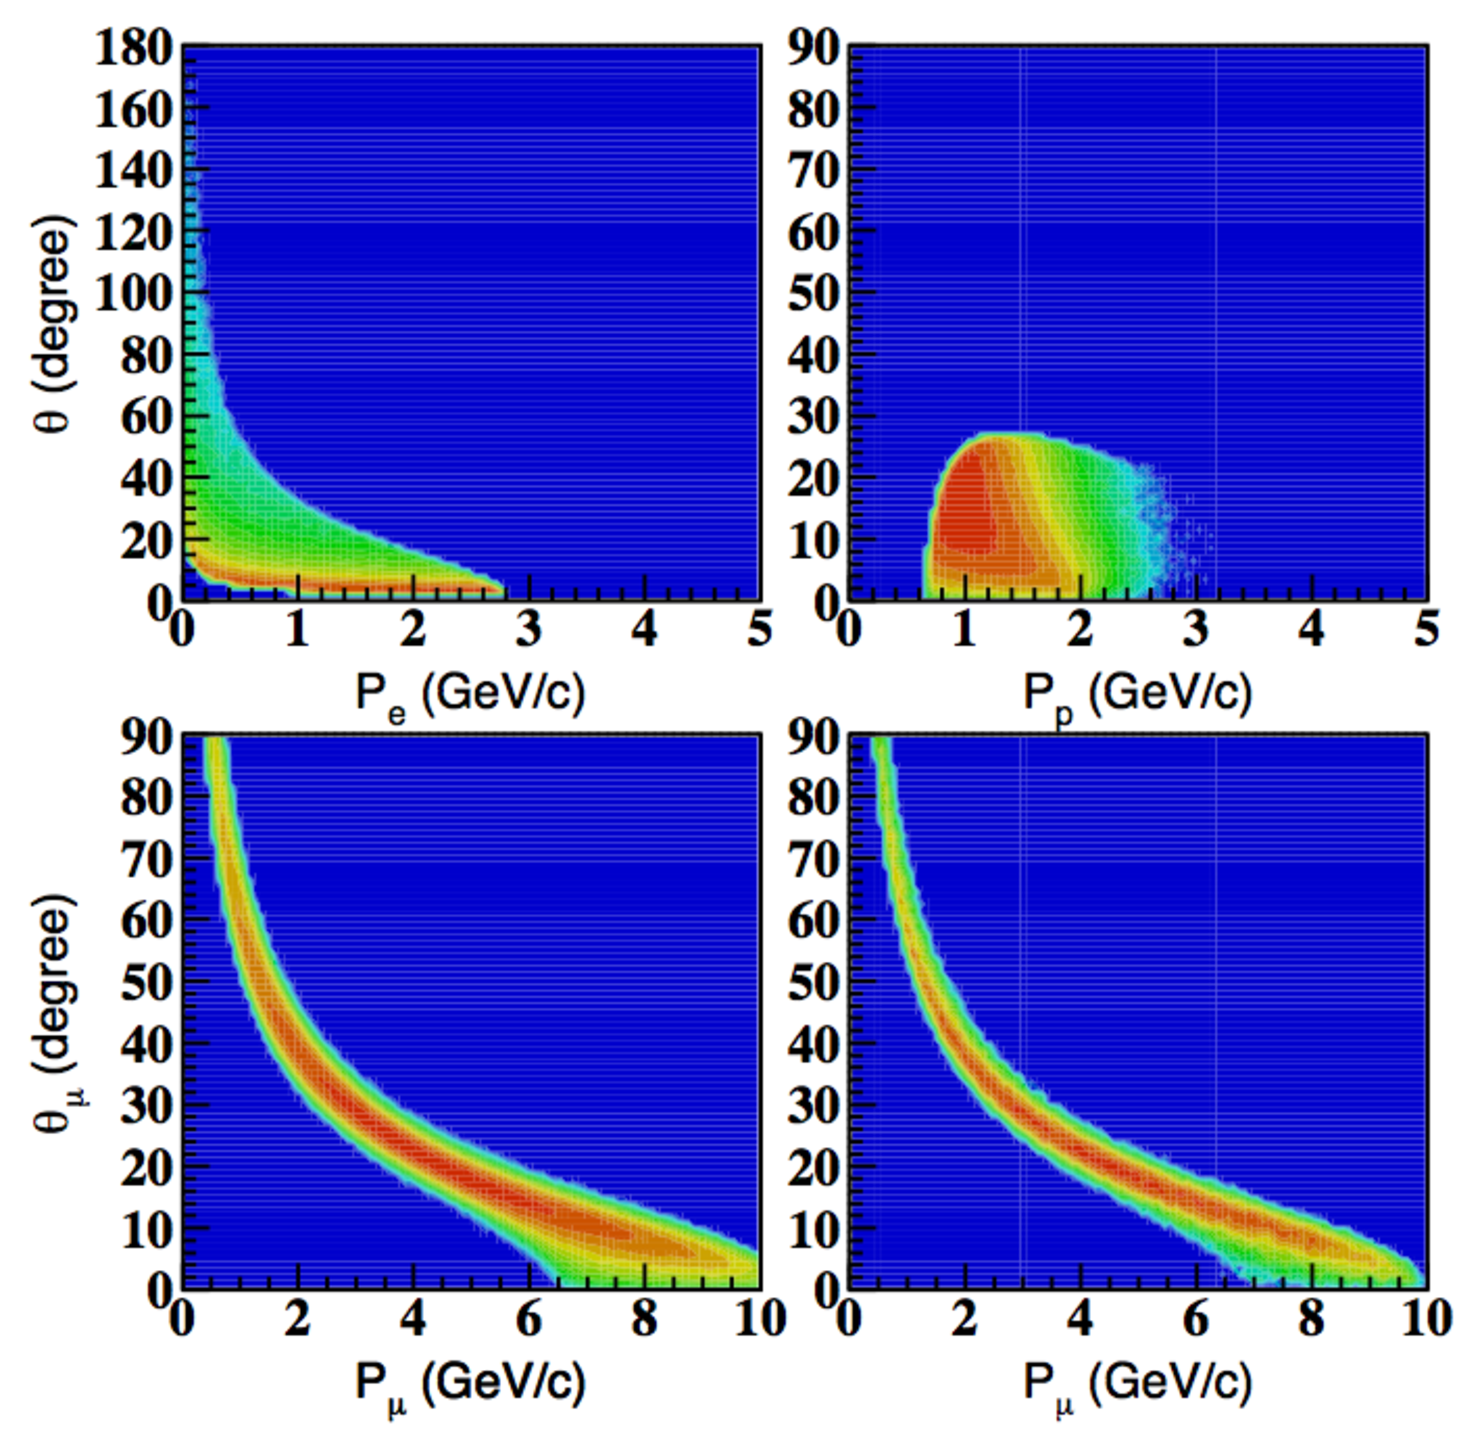
\includegraphics[width=0.8\textwidth]{jpsi_kine.pdf}
\caption{Kinematics of the scattered electron, recoil proton, and the decay muons for the reaction $ep\to e^\prime p^\prime J/\Psi $. In the bottom-right panel angular-momentum distribution of muons is shown for events where electron momentum is $p>0.5$ GeV and is in the scattering angular range $5^\circ <\theta<35^\circ$.}
\label{fig:jp_kine}
\end{center}
\end{figure}

\begin{figure}[htbp]
\begin{center}
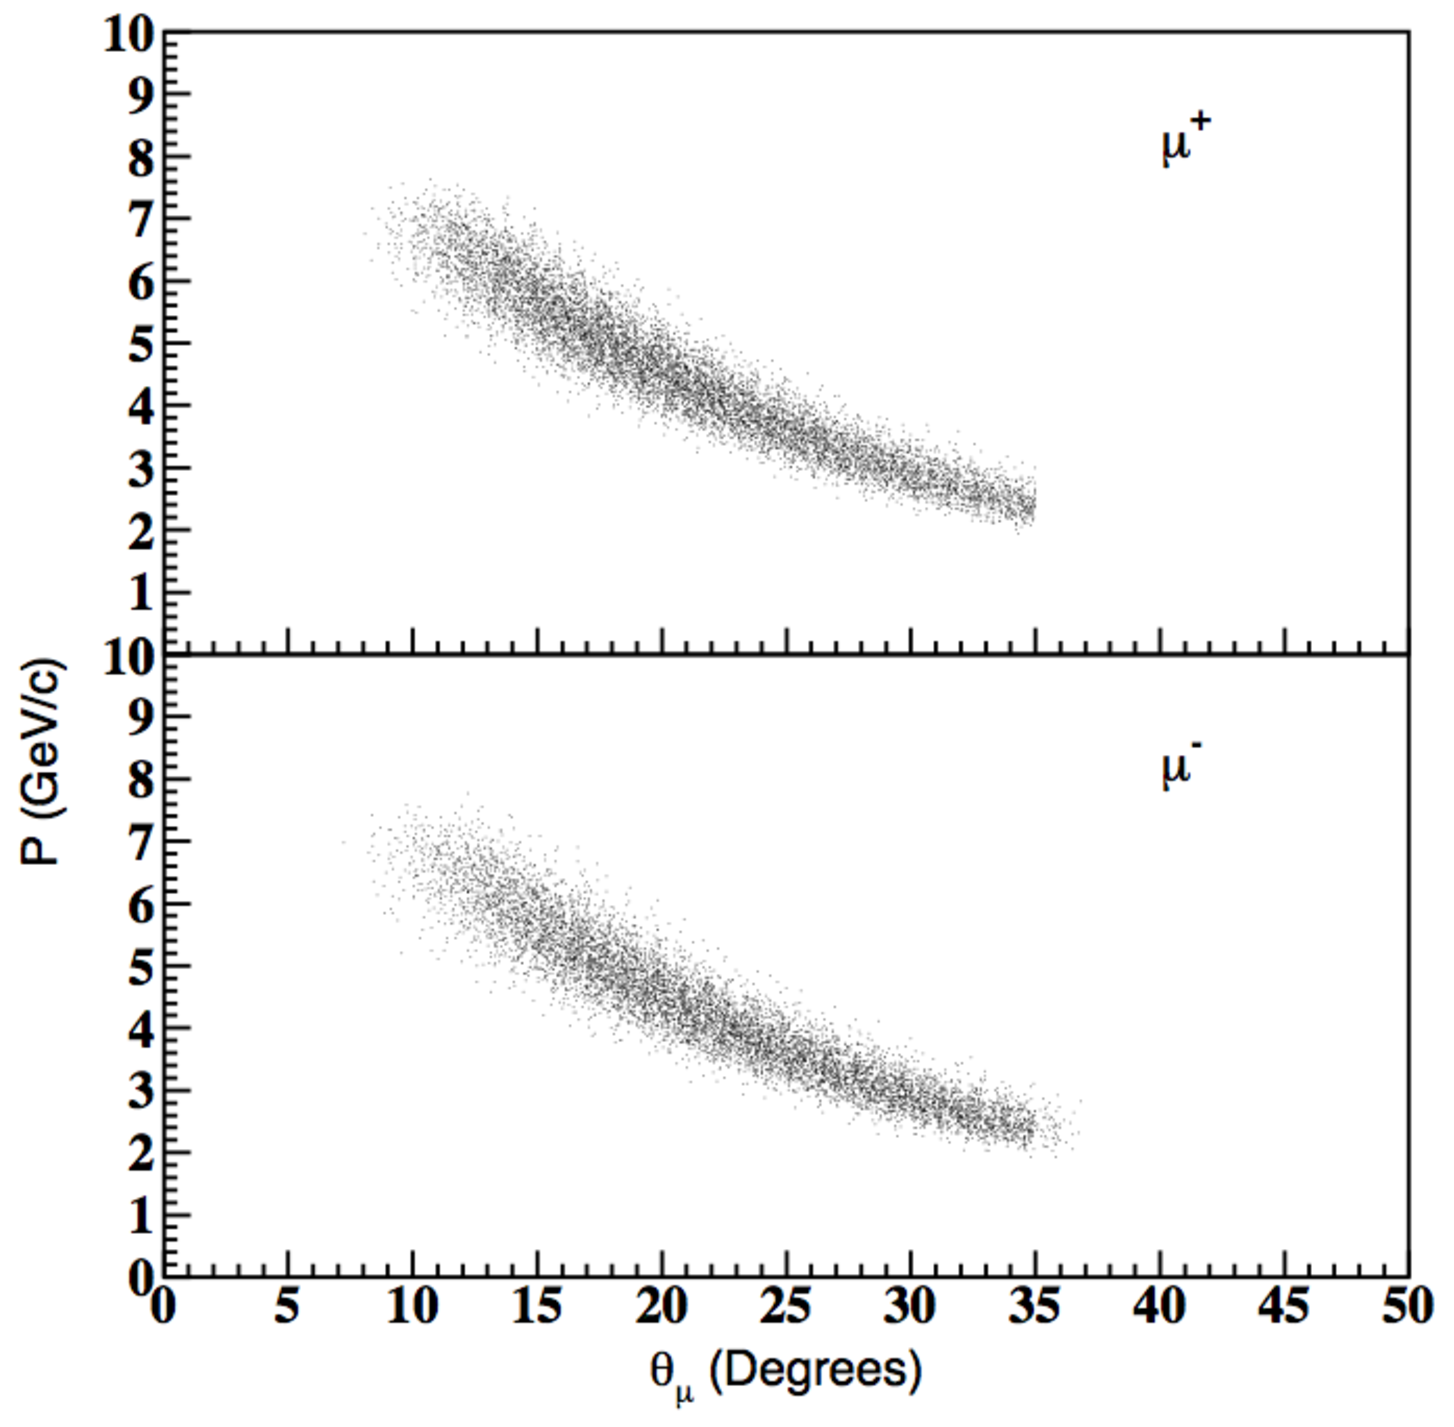
\includegraphics[width=0.6\textwidth]{jpsi_muon_p_theta_detected.pdf}
\caption{Angular-momentum distributions of $\mu^+$ (top) and $\mu^-$ bottom detected in the CLAS12 FD. }
\label{fig:jp_mukine}
\end{center}
\end{figure}

Since the proton will not be detected, when exclusivity is required the missing momentum analysis  of the $e\mu^+\mu^-$ final state will be performed to select events in the reaction $ep\to e^\prime p^\prime J/\Psi$, after identifying the $J/\Psi$ in the invariant mass of the muon pairs. For this, the mass (invariant and missing) resolution  will play an important role in identification of the reaction.  In Fig.\ref{fig:jp_mres} the expected resolutions for invariant and missing masses are shown. These distributions have been calculated using reconstructed, smeared, 3-momenta of the electron, $\mu^+$ and $\mu^-$ using the angular and momentum resolutions described above. Both distributions are fitted with Gaussian function. The standard deviations (mass resolutions) for both are $\sim 47$ MeV, indicating that identification of the J/$\Psi$ or the missing recoil proton is sufficient. 

\begin{figure}[htbp]
\begin{center}
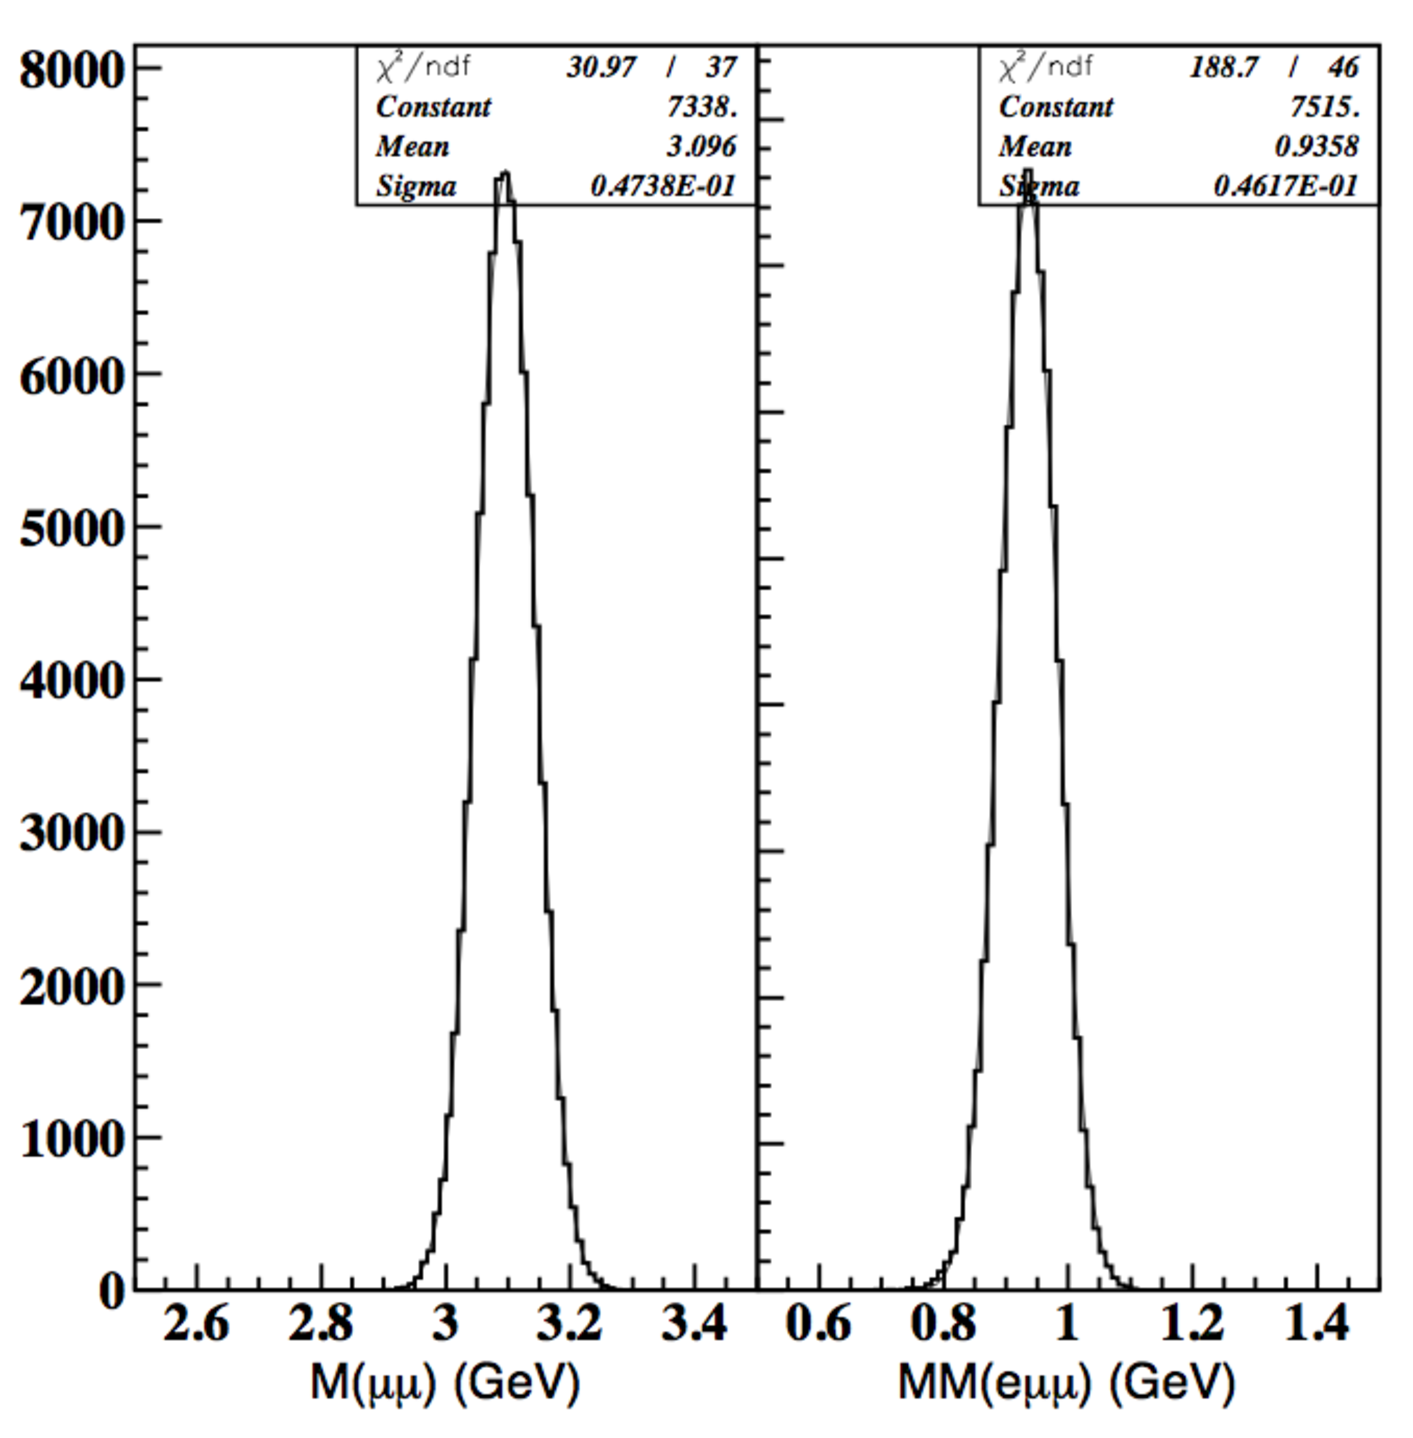
\includegraphics[width=.5\textwidth]{jpsi_minv_mmis_resolutions.pdf}
\caption{Expected mass resolutions: left the invariant mass of muon pairs, right the missing mass squared for the reaction $ep\to e^\prime \mu^+ \mu^- (p)$.}
\label{fig:jp_mres}
\end{center}
\end{figure}

As will be described below, the goal of the J/$\Psi$ electroproduction study will be the measurements of the t-dependence of the cross section in three bins of Q$^2$, $0.1<$Q$^2 <0.3$ GeV$^2$, $0.3<$Q$^2 <1.$ GeV$^2$, and $1<$Q$^2 < 2.5$ GeV$^2$. Therefore, our studies of the acceptances are also in these three bins of Q$^2$. The t-dependence of acceptances shown in Fig.\ref{fig:jp_acc}. The average acceptance for detection of (e$\mu^+\mu^-$) is about $\sim 3\%$, somewhat lower for lowest Q$^2$ bin. These acceptance values are used to calculate expected  rates. 

\begin{figure}[htbp]
\begin{center}
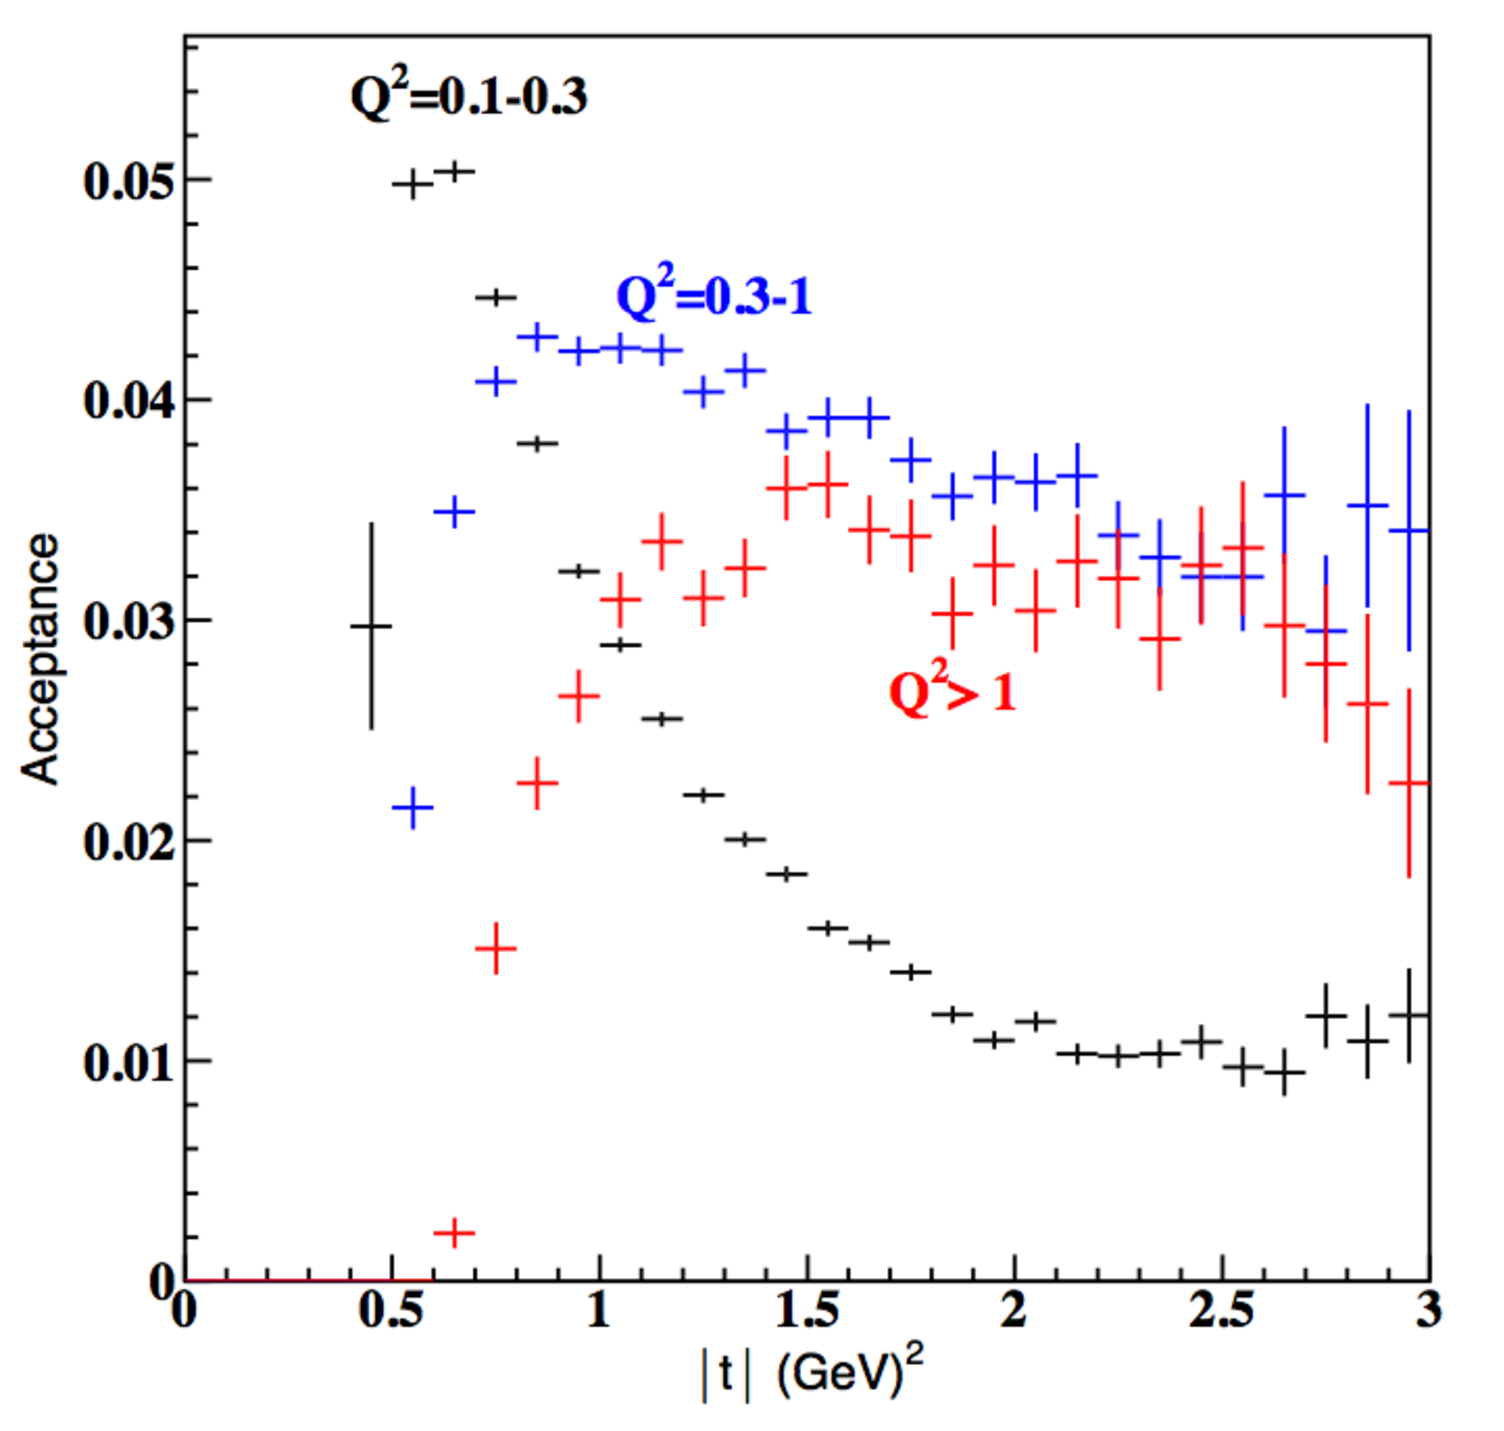
\includegraphics[width=.65\textwidth]{jpsi_t_acceptance_3Q2.pdf}
\caption{Acceptances as a function of $t$ for three Q$^2$ bins.}
\label{fig:jp_acc}
\end{center}
\end{figure}




%\clearpage


\subsubsection{Rates and projected results}
\indent

 Using photoproduction cross sections, $d\sigma/dt$,  from calculations presented in the proposal for the experiment E12-12-001 \cite{e1212001}, first $\sigma_T$ and $\sigma_L$ are calculated as described in Eqs. \ref{eq:st} and \ref{eq:sl}, then the virtual photon flux, $\Gamma_W$ (Eq.\ref{eq:flux}), and the cross section d$\sigma$/dW/dQ$^2$/dt as presented in Eq.\ref{eq:cse} using the bin average kinematical points (W, Q$^2$, and $t$). In Fig.\ref{fig:jp_rates} expected rates as a function of $t$ are shown for three Q$^2$ bins. The projected t-dependances of measured cross section is shown in Fig.\ref{fig:jp_xs}. The error bars on the points are expected statistical accuracy as shown in Fig.\ref{fig:jp_rates}.  
 
\begin{figure}[htbp]
\begin{center} 
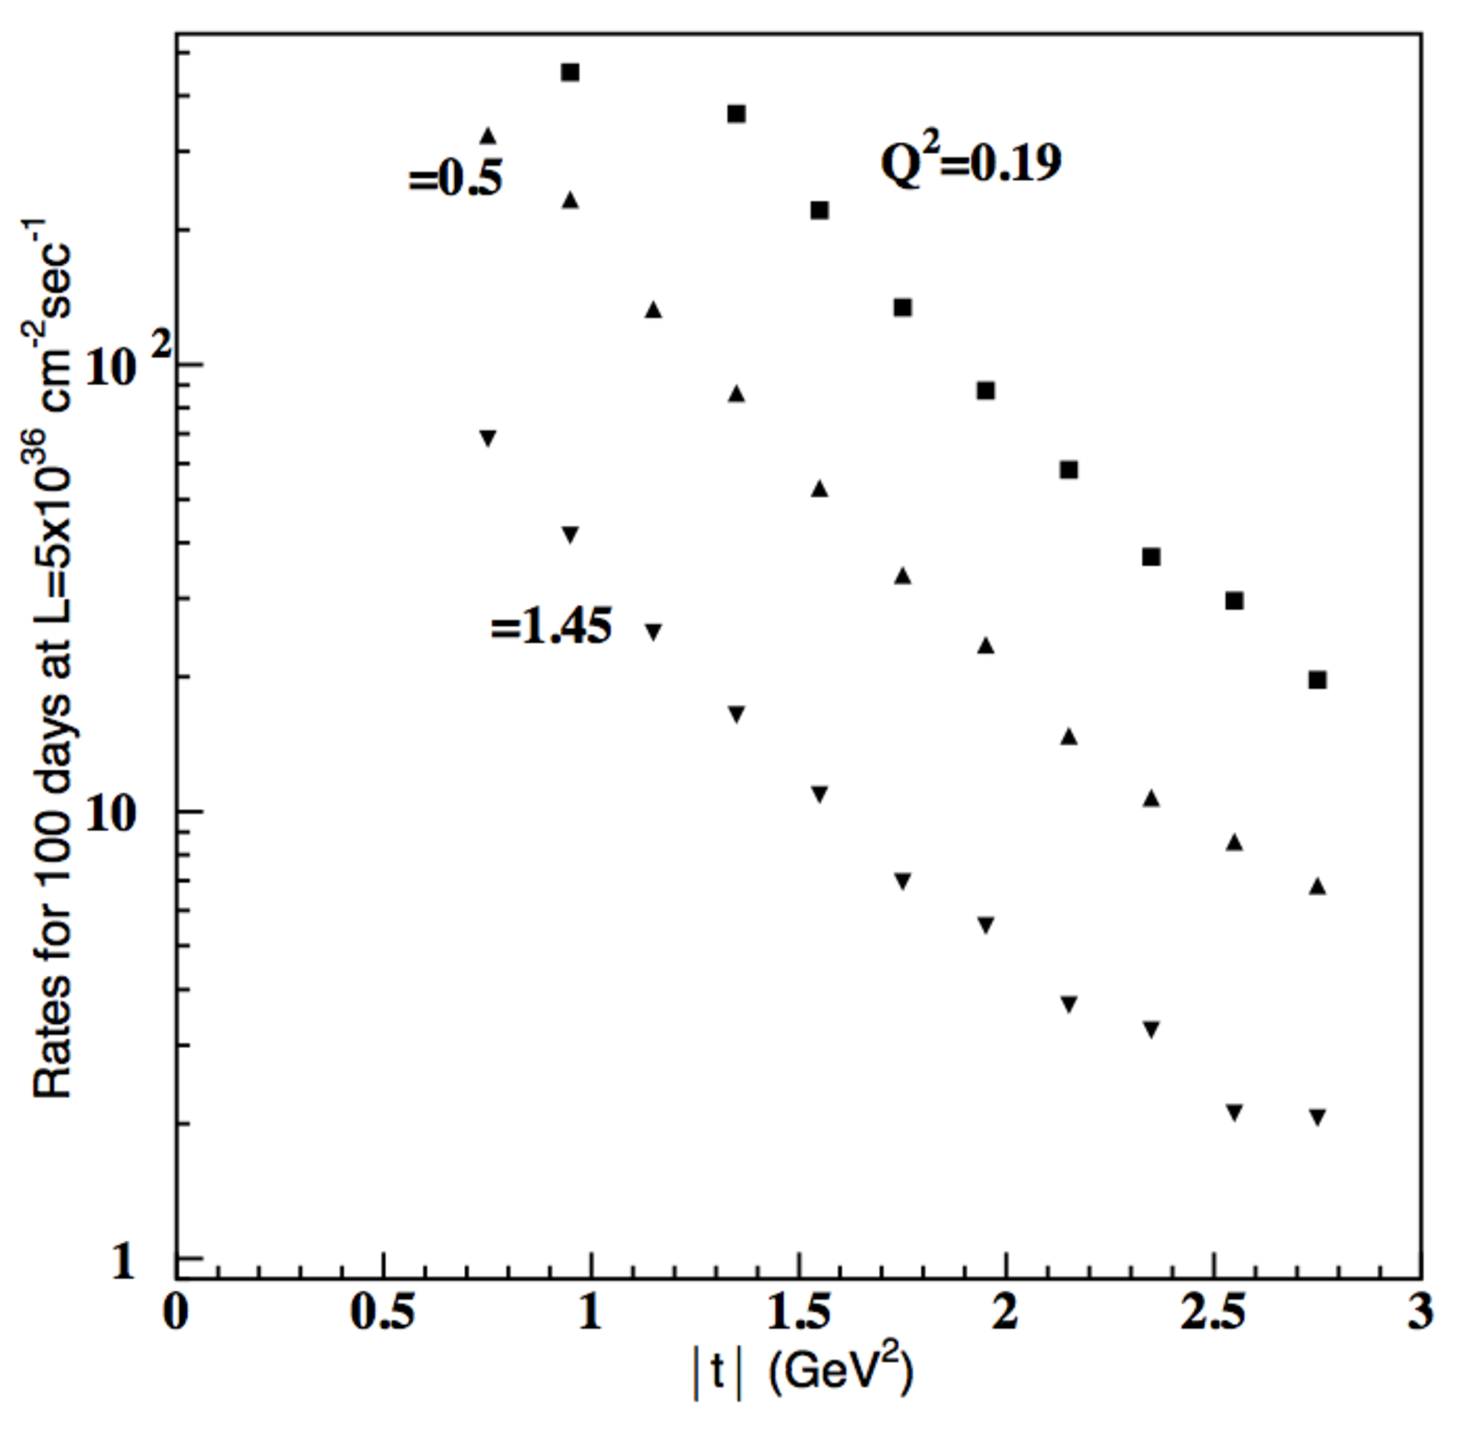
\includegraphics[width=0.65\textwidth]{jpsi_rates_3q2.pdf}
\caption{The expected rates as a function of t  for three Q$^2$ bins for $4.025 < W < 4.525$ GeV. Rates correspond to 100 days of running at luminosity of $5\times10^{36}$ cm$^{-2}$ sec$^{-1}$.}
\label{fig:jp_rates}
\end{center}
\end{figure}

 \begin{figure}[htbp]
\begin{center} 
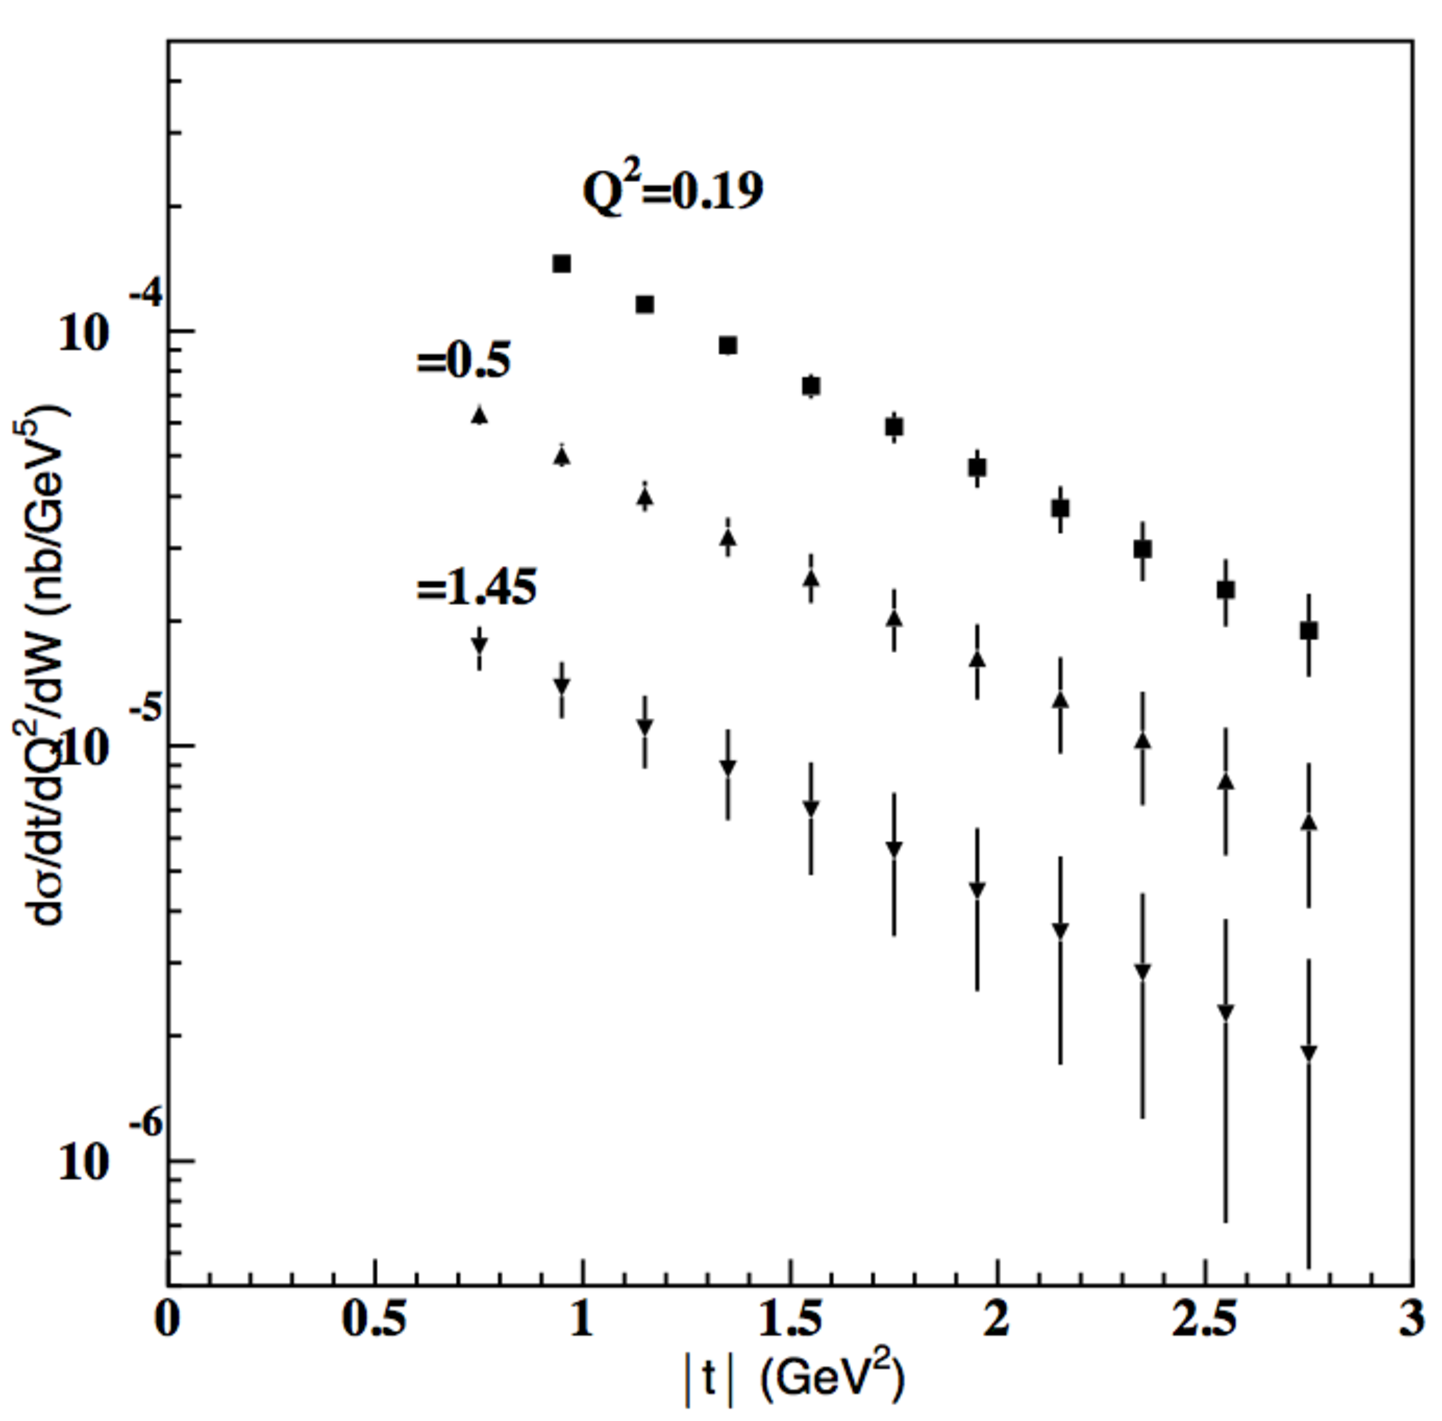
\includegraphics[width=0.65\textwidth]{jpsi_xs_3q2_errors.pdf}
\caption{The expected rates as a function of t  for three Q$^2$ bins for $4.025 < W < 4.525$ GeV. Rates correspond to 100 days of running at luminosity of $5\times10^{36}$ cm$^{-2}$ sec$^{-1}$.}
\label{fig:jp_xs}
\end{center}
\end{figure}


 
 


\section{Beam Time Estimate}

\section{Summary}

\begin{thebibliography} {999}

%\begin{thebibliography}{999}

\bibitem{goeke} K. Goeke, M. V. Polyakov and M. Vanderhaeghen,
Prog.\ Part.\ Nucl.\ Phys. {\bf 47} 401 (2001).
\bibitem{revdiehl}
M. Diehl, Phys.  Rept. {\bf 388} 41 (2003).
\bibitem{revrady}
A.V. Belitsky, A.V. Radyushkin, Phys. Rept. {\bf 418} 1 (2005).
\bibitem{rpp} 
M. Guidal, H. Moutarde and M. Vanderhaeghen, Rept. Prog. Phys. {\bf 76} 
066202 (2013).
\bibitem{Berger:2001xd}
  E.~R.~Berger, M.~Diehl and B.~Pire,
  Eur.\ Phys.\ J.\ C {\bf 23} 675 (2002).
\bibitem{Goritschnig} 
  A.~T.~Goritschnig, B.~Pire and J.~Wagner,
  %``Timelike Compton scattering with a linearly polarized photon beam,''
  arXiv:1404.0713 [hep-ph].
\bibitem{Boer:2015hma}
  M.~Bo�r, M.~Guidal and M.~Vanderhaeghen,
  %``Single and double polarization observables in timelike Compton scattering off proton,''
  arXiv:1501.00270 [hep-ph].
  
  \bibitem{Ji:1996nm} 
  Ji X D 1997 
  Deeply virtual Compton scattering 
  {\it Phys.\ Rev.\ D} {\bf 55} 7114 

\bibitem{marcprl2}
M. Vanderhaeghen, P.A.M. Guichon, M. Guidal, 
Phys. Rev. D {\bf 60}, 094017 (1999). 

\bibitem{carlos} C. Mu\~noz Camacho et al., Phys.\ Rev.\ Lett. {\bf 97}, 262002 (2006).
\bibitem{Jo:2015ema}
  H.~S.~Jo {\it et al.}  [CLAS Collaboration],
  %``Cross sections for the exclusive photon electroproduction on the proton and Generalized Parton Distributions,''
  arXiv:1504.02009 [hep-ex].

\bibitem{fx} F.-X. Girod et al., Phys.\ Rev.\ Lett. {\bf 100}, 162002 (2008).
\bibitem{shifeng} S. Chen et al., Phys. Rev. Lett. {\bf 97}, 072002 (2006).
\bibitem{erin} E. Seder et al., Phys. Rev. Lett. {\bf 114} 3 (2015).
\bibitem{Pisano:2015iqa}
  S.~Pisano {\it et al.}  [CLAS Collaboration],
  %``Single and double spin asymmetries for deeply virtual Compton scattering measured with CLAS and a longitudinally polarized proton target,''
  Phys.\ Rev.\ D {\bf 91} (2015) 5,  052014
  [arXiv:1501.07052 [hep-ex]].
  
  \bibitem{fitmuller} K. Kumericki and D. M\"uller, 
Nucl.\ Phys.\ B {\bf 841}, 1 (2010).
\bibitem{herve}
H.~Moutarde, Phys.\ Rev.\ D {\bf 79}, 094021 (2009).
\bibitem{fitmick} M. Guidal, Eur.\ Phys.\ J.\ A {\bf 37}, 319 (2008)
[Erratum-ibid.A40:119,2009]. 
\bibitem{fithermes} M. Guidal and H. Moutarde, Eur.\ Phys.\ J.\ A {\bf 42}, 
71 (2009).
\bibitem{fittsa} M. Guidal, Phys. Lett. B {\bf 689} (2010) 156.
\bibitem{fitall} M. Guidal, Phys. Lett. B {\bf 693} (2010) 17.
\bibitem{Guidal:2002kt}
  M.~Guidal and M.~Vanderhaeghen,
  %``Double deeply virtual Compton scattering off the nucleon,''
  Phys.\ Rev.\ Lett.\  {\bf 90} (2003) 012001
\bibitem{ddvcs_bm1} A. V. Belitskyand D. Mueller, Phys. Rev. Lett. {\bf 90}, 022001 (2003)
\bibitem{ddvcs_bm2}  A. V. Belitsky and D. Mueller,Phys. Rev.D {\bf 68}, 116005 (2003).
\bibitem{Muller:2012yq}
  D.~Mueller, B.~Pire, L.~Szymanowski and J.~Wagner,
  %``On timelike and spacelike hard exclusive reactions,''
  Phys.\ Rev.\ D {\bf 86} (2012) 031502
%\end{thebibliography}

\bibitem{fastmc} CLAS12 Fast Monte-Carlo simulator, 

/group/clas/clas\_cvs/12gev/fastmc/

\bibitem{fsgen} S. Stepanyan, Phase space event generator (Privet communications). 

\bibitem{HPS} M. Holtrtop, J. Jaros, and S. Stepanyan, Heavy Photon Experiment in Hall-B at Jefferson lab, E12-11-006 (2011).

\bibitem{lepto} CERN library program, Lepto651 and Jetset74 (2005).

\bibitem{vdm} J. Sakurai, Phys. Rev. Lett. 22, p981 (1966).

\bibitem{brodsky:2000zc} S.J. Brodsky, E. Chudakov, P. Hoyer, and J.M. Laget, Phys. Lett. B498, pp. 23-29 (2001).

\bibitem{e1212001} P. Nadel-Turonski et al., Timelike Compton Scattering and J/psi photoproduction on the proton in e+e- pair production with CLAS12 at 11 GeV, E12-12-001 (2012).

\bibitem{pdg} Particle Data Group, Physics Letter {\bf B667} (2008).


\end{thebibliography}

\end{document}